%\documentclass[preprint,authoryear,review,12pt]{elsarticle}
\documentclass{frontiersSCNS}
%% Use the option review to obtain double line spacing
%% \documentclass[preprint,review,12pt]{elsarticle}

%% Use the options 1p,two column; 3p; 3p,twocolumn; 5p; or 5p,twocolumn
%% for a journal layout:
%% \documentclass[final,1p,times]{elsarticle}
%% \documentclass[final,1p,times,twocolumn]{elsarticle}
%% \documentclass[final,3p,times]{elsarticle}
%% \documentclass[final,3p,times,twocolumn]{elsarticle}
%% \documentclass[final,5p,times]{elsarticle}
%% \documentclass[final,5p,times,twocolumn]{elsarticle}
\usepackage{enumerate}
\usepackage{color}
\usepackage{multirow,booktabs,ctable,array}
\usepackage{lscape}
\usepackage{parallel}
\usepackage{amsmath}
\usepackage{lineno}
\usepackage{ulem}
\usepackage{setspace}
\usepackage{listings}
\usepackage{float}
\usepackage{amssymb}

\usepackage{algorithm}
\usepackage{algpseudocode}
\usepackage[colorlinks=true,urlcolor=cyan]{hyperref}
\usepackage{soul,url,verbatim,outline}
\usepackage{amsmath,amssymb,amsfonts,graphicx,amsthm,colortbl}
\usepackage{graphicx,subfigure}
\usepackage{tabularx,ragged2e,booktabs}
\usepackage[usenames,dvipsnames]{xcolor}
\newcommand{\R}{{\bf R}}
\newcommand{\X}{{\bf X}}
\newcommand{\Xh}{{\hat{{\bf X}}}}
\newcommand{\x}{{\bf x}}
\newcommand{\Y}{{\bf Y}}
% \newcommand{\U}{{\bf U}}
\newcommand{\V}{{\bf V}}
\newcommand{\E}{{\bf E}}
\newcommand{\y}{{\bf y}}
\newcommand{\Z}{{\bf Z}}
\newcommand{\z}{{\bf z}}
\newcommand{\bSigma}{\boldsymbol \Sigma}
\newcommand{\vect}[1]{\mathbf{#1}}
\newcommand{\field}[1]{\mathbf{#1}}
\newcommand{\image}[1]{#1}
\newcommand{\I}{\image{I}}
\newcommand{\J}{\image{J}}
\renewcommand{\u}{\vect{u}}
\renewcommand{\v}{\vect{v}}
\renewcommand{\c}{\vect{c}}
\newcommand{\h}{\vect{h}}
\newcommand{\w}{\vect{w}}
\newcommand{\myphi}{\phi}
\newcommand{\mypsi}{\psi}
\newcommand{\D}{D}
\renewcommand{\d}{\nabla}
\newcommand{\dd}{\text{d}}
\newcommand{\p}{\partial}
\renewcommand{\L}{\Delta} % laplacian
\newcommand{\myS}{S}
\newcommand{\myR}{R}
\newcommand{\myE}{E}
\newcommand{\ld}{\langle}
\newcommand{\rd}{\rangle}
\newcommand{\tQ}{\mathcal{Q}}
\newcommand{\Id}{\text{Id}}
\newcommand{\tG}{{G}} % operator L
\newcommand{\Diff}{\text{Diff}}
\newcommand{\VV}{\mathcal{V}}
\newcommand{\opL}{\mathcal{L}}
\newcommand{\bs}{\boldsymbol}
\newcommand{\bsp}{$\substack{
   \rightsquigarrow \\
   b
  }$}
\newcommand{\mi}{$\substack{
   \approx \\
   \text{mi}
  }$}
\newcommand{\cc}{$\substack{
   \approx \\
   \text{cc}
  }$}
\newcommand{\tk}{~ITK$^{\text{4}}$~}
\newcommand{\tkt}{~ITK$^{\text{3}}$~}
\usepackage{amsmath,amssymb}
\usepackage{times}
\usepackage{setspace,verbatim}
\usepackage{epsfig}


\usepackage[english]{babel}


\floatstyle{plain}
\newfloat{command}{thp}{lop}
\floatname{command}{Command}

%\usepackage[nomarkers,notablist]{endfloat}

%% if you use PostScript figures in your article
%% use the graphics package for simple commands
%% \usepackage{graphics}
%% or use the graphicx package for more complicated commands
%% \usepackage{graphicx}
%% or use the epsfig package if you prefer to use the old commands
%% \usepackage{epsfig}

%% The amssymb package provides various useful mathematical symbols
%% The amsthm package provides extended theorem environments
% \usepackage{amsthm}


%% The lineno packages adds line numbers. Start line numbering with
%% \begin{linenumbers}, end it with \end{linenumbers}. Or switch it on
%% for the whole article with \linenumbers after \end{frontmatter}.
%% \usepackage{lineno}

%% natbib.sty is loaded by default. However, natbib options can be
%% provided with \biboptions{...} command. Following options are
%% valid:

%%   round  -  round parentheses are used (default)
%%   square -  square brackets are used   [option]
%%   curly  -  curly braces are used      {option}
%%   angle  -  angle brackets are used    <option>
%%   semicolon  -  multiple citations separated by semi-colon
%%   colon  - same as semicolon, an earlier confusion
%%   comma  -  separated by comma
%%   numbers-  selects numerical citations
%%   super  -  numerical citations as superscripts
%%   sort   -  sorts multiple citations according to order in ref. list
%%   sort&compress   -  like sort, but also compresses numerical citations
%%   compress - compresses without sorting
%%
%% \biboptions{comma,round}

% \biboptions{}

\providecommand{\OO}[1]{\operatorname{O}\bigl(#1\bigr)}

\graphicspath{{./Figures/}
              {./Results/}}

\long\def\symbolfootnote[#1]#2{\begingroup%
\def\thefootnote{\fnsymbol{footnote}}\footnote[#1]{#2}\endgroup}

    \usepackage{color}

    \definecolor{listcomment}{rgb}{0.0,0.5,0.0}
    \definecolor{listkeyword}{rgb}{0.0,0.0,0.5}
    \definecolor{listnumbers}{gray}{0.65}
    \definecolor{listlightgray}{gray}{0.955}
    \definecolor{listwhite}{gray}{1.0}

\newcommand{\lstsetcpp}
{
\lstset{frame = tb,
        framerule = 0.25pt,
        float,
        fontadjust,
        backgroundcolor={\color{listlightgray}},
        basicstyle = {\ttfamily\scriptsize},
        keywordstyle = {\ttfamily\color{listkeyword}\textbf},
        identifierstyle = {\ttfamily},
        commentstyle = {\ttfamily\color{listcomment}\textit},
        stringstyle = {\ttfamily},
        showstringspaces = false,
        showtabs = false,
        numbers = none,
        numbersep = 6pt,
        numberstyle={\ttfamily\color{listnumbers}},
        tabsize = 2,
        language=[ANSI]C++,
        floatplacement=!h,
        caption={},
        captionpos=b,
        }
}

\providecommand{\e}[1]{\ensuremath{\times 10^{#1}}}

\copyrightyear{}
\pubyear{}

\def\journal{Neuroscience}%%% write here for which journal %%%
\def\DOI{}
\def\articleType{Methods}
\def\keyFont{\fontsize{8}{11}\helveticabold }
\def\firstAuthorLast{Avants et al.} %use et al only if is more than 1 author
\def\Authors{Brian B. Avants$^{1}$, Nicholas J. Tustison$^{2}$, Michael
  Stauffer$^{1}$, Gang Song$^{1}$, Baohua Wu$^{1}$ and James C. Gee$^{1}$}
% Affiliations should be keyed to the author's name with superscript numbers and be listed as follows: Laboratory, Institute, Department, Organization, City, State abbreviation (USA, Canada, Australia), and Country (without detailed address information such as city zip codes or street names).
% If one of the authors has a change of address, list the new address below the correspondence details using a superscript symbol and use the same symbol to indicate the author in the author list.
\def\Address{
$^{1}$Penn Image Computing and Science Laboratory, University of Pennsylvania, Department of Radiology, Philadelphia, PA, USA \\
$^{2}$University of Virginia, Department of Radiology and Medical Imaging, Charlottesville, VA, USA 
}
% The Corresponding Author should be marked with an asterisk
% Provide the exact contact address (this time including street name and city zip code) and email of the corresponding author
\def\corrAuthor{Brian B. Avants}
\def\corrAddress{University of Pennsylvania, Department of Radiology,
  3600 Market St, Philadelphia, PA, 19104}
\def\corrEmail{avants@grasp.cis.upenn.edu}
\begin{document}
\onecolumn
\firstpage{1}

\title[ITKv4 Image Registration]{The Insight ToolKit Image
  Registration Framework}
\author[\firstAuthorLast ]{\Authors}
\address{}
\correspondance{}
\editor{}
\topic{}

\maketitle

%\linenumbers


\begin{comment}
\author{Brian B. Avants$^1$, Nicholas J. Tustison$^2$, Gang Song$^1$, Baohua Wu$^1$,
  Michael Stauffer$^1$, \\Matthew M. McCormick$^3$, Hans J. Johnson$^4$,
  James C. Gee$^1$ \\and the
  $^5$\href{http://www.insightsoftwareconsortium.org/}{Insight Software Consortium}\\
$^1$Penn Image Computing and Science Lab \\ Dept. of Radiology \\University of
  Pennsylvania, Philadelphia, PA, 19104\\ 
  $^2$Dept. of Radiology and Medical Imaging, \\ University of Virginia,
  Charlottesville, VA 22903\\
  $^3$Department of Psychiatry \\The University of Iowa, IA 52242\\
  $^4$Kitware, Inc. \\ Clifton Park, NY 12065\\
  $^5$\href{http://www.insightsoftwareconsortium.org/}{http://www.insightsoftwareconsortium.org/}}
\end{comment}
\begin{abstract}
Publicly available scientific resources help establish evaluation
standards, provide a platform for teaching and improve
reproducibility.  Version 4 of the Insight ToolKit (\tk) seeks to
establish new standards in publicly available image registration
methodology.  \tk makes several advances in comparison to previous
versions of ITK.  \tk supports both multivariate images and objective
functions; it also unifies high-dimensional (deformation field) and
low-dimensional (affine) transformations with metrics that are
reusable across transform types and with composite transforms that
allow arbitrary series of geometric mappings to be chained together
seamlessly.  Metrics and optimizers take advantage of multi-core
resources, when available.  Furthermore, \tk reduces the
parameter optimization burden via principled heuristics 
that automatically set scaling across disparate parameter types
(rotations versus translations).  A related approach also constrains
steps sizes for gradient-based optimizers.  The result is that tuning for different metrics and/or image
pairs is rarely necessary allowing the researcher to more easily focus
on design/comparison of registration strategies.  In total, the \tk contribution is intended as a structure to
support reproducible research practices, will provide a more extensive
foundation against which to evaluate new work in image registration
and also enable application level programmers a broad suite of tools
on which to build.  Finally, we contextualize this work with a reference registration
evaluation study with application to pediatric brain labeling.\footnote{This work is supported by National
Library of Medicine sponsored ARRA stimulus funding.}
\end{abstract}

\section{Introduction}
As image registration methods mature---and their capabilities become
more widely recognized---the number of applications increase
\citep{Rueckert1999,2004,Shelton2005,Miller2005,Chen2008,Cheung2009,Baloch2009,Peyrat2010,Metz2011,Kikinis2011,Fedorov2011,Murphy2011}.
Consequently, image registration transitioned from being a field of active research, and few applied results, to a
field where the main focus is translational.  Image registration is
now used to derive quantitative biomarkers from images
\citep{Jack2010a}, plays a major role in business models and clinical
products (especially in radiation oncology) \citep{Cheung2009}, has led
to numerous new findings in studies of brain and behavior \citep[e.g.,][]{Bearden2007} 
and is a critical component in applications in
pathology, microscopy, surgical planning and more
\citep{Shelton2005,Miller2005,Floca2007,Chen2008,Cheung2009,Peyrat2010,Kikinis2011,Murphy2011}.
Despite the increasing relevance of image registration across
application domains, there are relatively few reference algorithm
implementations available to the community.  Furthermore, these
resources have become critical to setting performance standards in
international challenges that evaluate ``real world'' registration
scenarios (see, for instance, the SATA 2013 and BRATS 2013 challenges
at MICCAI in Nagoya, Japan). 

% \cite{Jenkinson2001,Christensen1996,Rueckert1999,Yoo2002,Ackerman2003,2004,Shelton2005,Wolf2005,Miller2005,Floca2007,Chen2008,Khan2008,Cheung2009,Vercauteren2009,Baloch2009,Klein2010,Peyrat2010,Taka2011,Metz2011,Kikinis2011,Fedorov2011,Murphy2011,Avants2011}.

% itk 

% ideas 

% Taka2011,Metz2011,,Fedorov2011,,}.
% {\bf How is image registration applied?}

% {\bf What role has ITK filled in the registration world?}  

One source of benchmark methodology is the Insight ToolKit (ITK)
\citep{Yoo2002,Ackerman2003}, which marked a significant contribution to
medical image processing when it first emerged at the turn of the millennium.
Since that time, ITK has become a standard-bearer for image
processing algorithms and, in particular, for image registration
methods.  In a review of ITK user interests, image registration was cited as the 
most important
contribution of ITK (personal communication with Terry Yoo).  Numerous papers use ITK
algorithms as standard references for implementations of Demons
registration and mutual information-based affine or B-Spline
registration \citep{2004,Shelton2005,Floca2007,Chen2008,Cheung2009}.
Multiple toolkits extend ITK registration methods in unique ways.
Elastix provides very fast and accurate B-Spline registration
\citep{Klein2010,Murphy2011}.  The diffeomorphic demons is a fast/efficient
approximation to a diffeomorphic mapping \citep{Vercauteren2009}.  
ANTs provides both flexibility and high average performance
\citep{Avants2011}.  The BRAINSFit algorithm is integrated into Slicer
for user-guided registration \citep{Kikinis2011}.
Each of these toolkits has both strengths and weaknesses
\citep{Klein2010,Murphy2011} and was enabled by an ITK core.    
%  What papers use ITK as a standard for comparison?  What other software builds on ITK registration?

%How does the v4 registration framework build on the past?  What does it contribute that's new?  
% What is it? Why were these the tools we chose to contribute?  
% {\bf \tk Registration: What it is.}
The Insight ToolKit began a major refactoring effort in 2010.
The refactoring aimed to both simplify and extend the techniques available in version
3.x with methods and ideas from a new set of prior work
\citep{Jenkinson2001,Christensen1996,Rueckert1999,Miller2005,Peyrat2010,Avants2011}.
To make this technology more accessible, \tk unifies the dense
registration framework (displacement field, diffeomorphisms)
with the low-dimensional (B-Spline, affine, rigid) framework by
introducing composite transforms, deformation field transforms and
specializations that allowed these to be optimized efficiently.  A sub-goal set for \tk was to simplify
parameter setting by adding helper methods that use well-known
principles of image registration to automatically scale transform
components and set optimization parameters.  \tk transforms are also
newly applicable to objects such as vectors and tensors and will take into account covariant geometry if
necessary.  Finally, \tk reconfigures the registration framework
to maximize multi-threading resources where possible.
The revised registration framework within ITK is more thoroughly
integrated across transform models, is thread-safe and provides
broader functionality than in prior releases. 

% graceful failure of an algorithm.  Should not be catastrophic. A nice feedback loop for software.  

%{\bf procedure: 1. clinicians are conservative.  2.  first, prove robustness.  3. provide useful and encouraging feedback.  4. fail gracefully when do fail.   }

% good average performance versus good performance on a given dataset.

David Donoho once commented (in paraphrase) that academic publications
are merely ``advertisements'' for the real work which is constituted
by the ``complete instruction set'' that produces the results reported
in the publication \citep{buckheit1995}.  The first part of the remainder 
of this document will provide an
``advertisement'' for the ITK framework and summarize its evolution
from \tkt to \tk.  We then detail potential applications of this \tk
framework in the context of a general nomenclature.  While this work is indeed incomplete, in the
sense of Donoho, we refer to source code and data when relevant.
Furthermore, section \ref{sec:applications} shows a series of
reproducible examples of \tk in action.  Several
areas relevant to neuroinformatics are highlighted in these examples: optimal template
construction, ``challenging'' registration scenarios involving brain
mapping in the presence of lesions or resection, registration when
initialization priors are weak, asymmetry analyses, functional MRI and
non-traditional registration strategies are all highlighted.  We also
establish performance benchmarks for the current \tk registration, in
comparison to a method developed for \tkt, via
a standard brain labeling task.  Finally, we discuss future developments
in the framework.

\section{Materials and Methods}
\subsection{Overview of the unified framework}
The overall purpose of the registration refactoring for \tk was to
simplify the user experience and to accelerate and improve
performance. Here, we summarize how \tk works toward these goals.
\begin{figure}[t]
\begin{center}
\begin{tabular}{c}
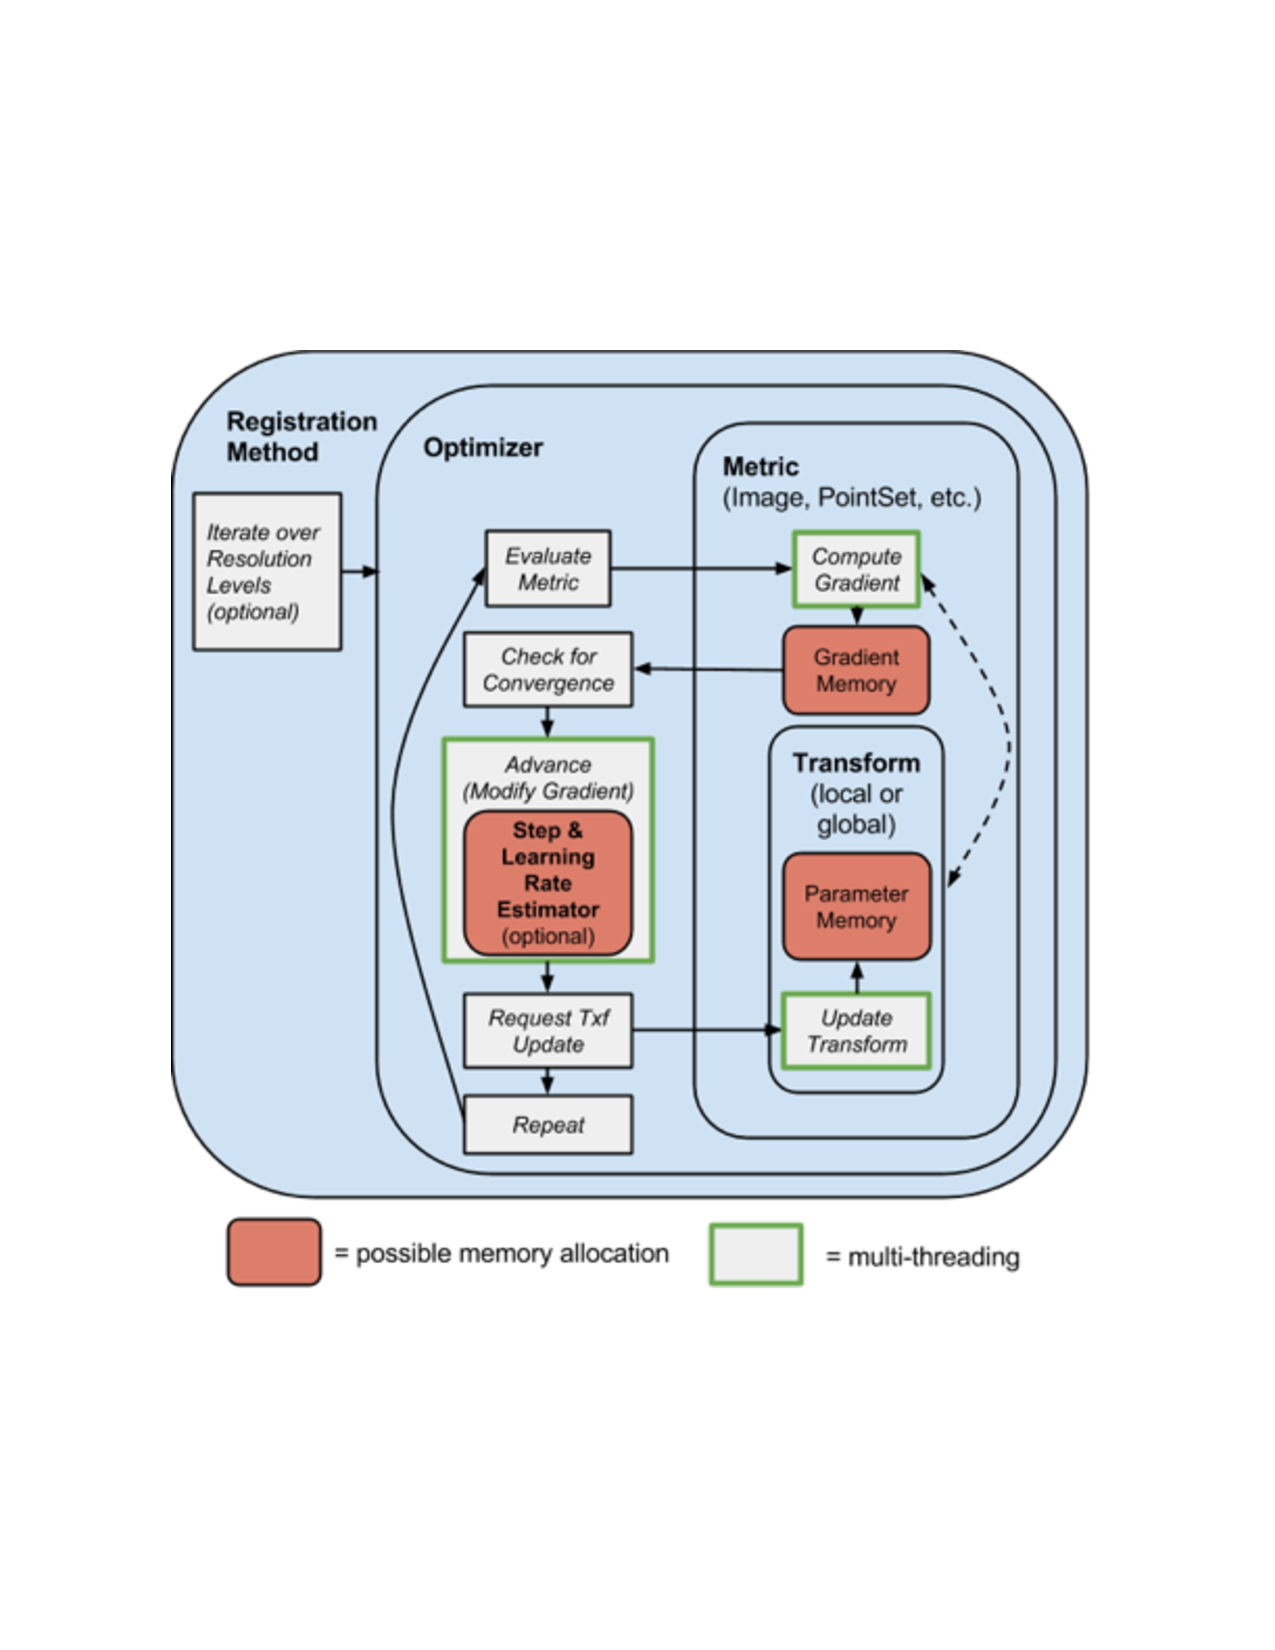
\includegraphics[width=5in]{figs/software_design.pdf}
\end{tabular}
\caption{A schematic overview of the
  prototypical \tk registration method.  This design is overall similar to
  that of \tkt.  A few key components differ:  (1) optimizers require that
  transforms update themselves; (2) metrics and optimizers are
  multi-threaded; (3) memory is shared across both optimizers and metrics,
greatly increasing efficiency; (4) automated (usually hidden) parameter
estimators are available; (5) transforms may include high-dimensional
deformation fields.  One additional difference (not shown) is that ``fixed''
images may also have a transformation, although this is not modified
by the optimizer.}
\label{fig:softw}
\end{center}
\end{figure}
\subsubsection{Core Software Components.} Figure~\ref{fig:softw} sketches the \tk architecture at a high level.
Registration applications are known as ``registration methods'' as
they were in \tkt.  The methods, with source contained in \tk's \texttt{RegistrationMethodsv4}
directory, hold together the different
subcomponents that make a working instantiation of a registration
strategy.  These subcomponents include the optimization technique (in
the \texttt{Optimizersv4} directory), the
metric measuring the registration quality\footnote{All \tk metrics
  are set to be minimized.  For instance, the
  \texttt{itkMattesMutualInformationImageToImageMetricv4} returns negative mutual information.} (the \texttt{Metricsv4} directory), the images or other data
objects that enter the metric and the parameters that are being
optimized.  The parameters are usually defined by a geometric
transformation but may point to other relevant objects.  Any of \tk's
transformations may be optimized by the framework.  New
transformations, relative to \tkt, include the
\texttt{DisplacementField} transforms that are useful for
engendering Demons or B-Spline registration strategies.  New
\texttt{VelocityField} transforms are also available.  A typical
application developer would employ all of these components.  A good
starting point for new users who wish to see how these tools work
together, in source code, is found in the tests.  For instance, see the
files
\texttt{itkTimeVaryingBSplineVelocityFieldImageRegistrationTest.cxx}
for an example of a B-Spline diffeomorphism application,
\texttt{itkSyNImageRegistrationTest.cxx} to see SyN in \tk and
\texttt{itkSimpleImageRegistrationTest2.cxx} for a more basic example.

% \textcolor{red}{The paper assumes a high-level of familiarity with the ITKv3 and ITKv4 framework. It would be helpful for readers who have little or limited familiarity with the software framework, if the paper contains a brief overview of the registration framework (the classes and the primary methods). For example, how methods such as ComputeJacobian... would fit in the overall registration framework would be unclear to a basic ITK user.}

Several usability goals spurred \tk development.  We summarize these here.

\subsubsection{Image registration should be achievable in one step.}
This overarching goal is best illustrated by \texttt{RegistrationMethodsv4} in which a user may string
together a series of registration tools to perform (for instance) a
translation registration, followed by an affine registration, followed
by a diffeomorphic mapping each of which might use a different image
similarity metric.  The different transforms are accumulated in the
new \texttt{itkCompositeTransform} which chains transforms together as in Figure~\ref{fig:composite}.
Thus, this
framework provides unprecedented ability to perform complex and staged
registration mappings.  Furthermore, the framework’s automated
parameter scaling, \texttt{itkRegistrationParameterScalesEstimator}, 
vastly reduces the difficulty of tuning parameters for different
transform/metric combinations.  

\subsubsection{ITK Transforms should be unified.}
Each ITK$^4$ transform now has either global support (affine
  transform) or local (or compact) support (a displacement field transform).   If
  any map in a composite transform has global support then the
  composite transform has global support.  Both ``fixed'' and ``moving'' images may have initial
  transforms.  This allows one to reduce ``registration bias'' that
  may be induced by asymmetric interpolation \citep{Yushkevich2010a}. 

\subsubsection{Registration mappings should be applicable to a number of popular data
types, including DTI.}  Our revisions to the \tkt transform hierarchy
validated and extended the \tkt transforms for thread safety and
applicability to not only vectors but also tensors.  Reorientation
steps necessary for diffusion tensor mappings are now included in
\tk.  

\subsubsection{Affine and deformable similarity metrics should look as similar as possible.}
The \texttt{Metricsv4} framework supports this goal in that it is as trivial to
implement a “mutual information” Demons algorithm as it is to
implement a “sum of squared differences” BSpline or affine
registration algorithm.  Thus, full “plug-and-play” support exists
across transforms.   


\subsubsection{Users should be able to combine multiple similarity metrics, some of which may operate on different data types.}
This is achievable with the existing \texttt{itkMultiGradientOptimizerv4}
through the multivariate \texttt{itkObjectToObjectMultiMetricv4} or
through the multi-channel traits
(\texttt{itkVectorImageToImageMetricTraitsv4}) that allow metrics to deal with
multi-channel pixels, all of which were contributed for \tk.  The
\texttt{itkObjectToObjectMultiMetricv4} was used in our winning entry
of the SATA 2013 ``dog leg'' challenge. 

\subsubsection{Optimizers and transformations should interact flexibly.}
\texttt{Optimizersv4} includes optimizers that are applicable to both linear and deformable transformations, which include convergence monitoring and enable 2nd order optimization (\texttt{itkQuasiNewtonOptimizerv4}), multiple objective optimization (\texttt{itkMultiGradientOptimizerv4}), or global optimization (\texttt{itkMultiStartOptimizerv4}).  

\subsubsection{GPU and multi-core acceleration will open up new applications for image registration.}
See \texttt{GPUPDEDeformable} for a GPU example.  Furthermore, the new metric framework $N$ cores to accelerate metric, gradient and optimization steps.  A recent real-world application of the new Insight ToolKit implementation of the symmetric normalization algorithm showed a speed-up of almost a factor of six when comparing single core to eight core execution time. This speed-up is achieved by multi-threading the similarity metric, the gradient descent update, the regularization terms and the composition components of the method. Thus, every essential step exploits intrinsic parallelism in the algorithm. Decreased execution time means more rapid turnaround for users, faster turn-around in testing and higher throughput on large-scale computing tasks.  

\subsubsection{Improve memory efficiency in optimization framework.}
Memory optimizations are critical for efficient use of large local transforms.
In \tk, transform parameters are no longer copied within the optimizer, but rather left in-place in transform. 
Metric gradient memory is shared between optimizer and metric, and modifications by the optimizer  are done in place when possible.
\begin{figure}[t]
\begin{center}
\begin{tabular}{c}
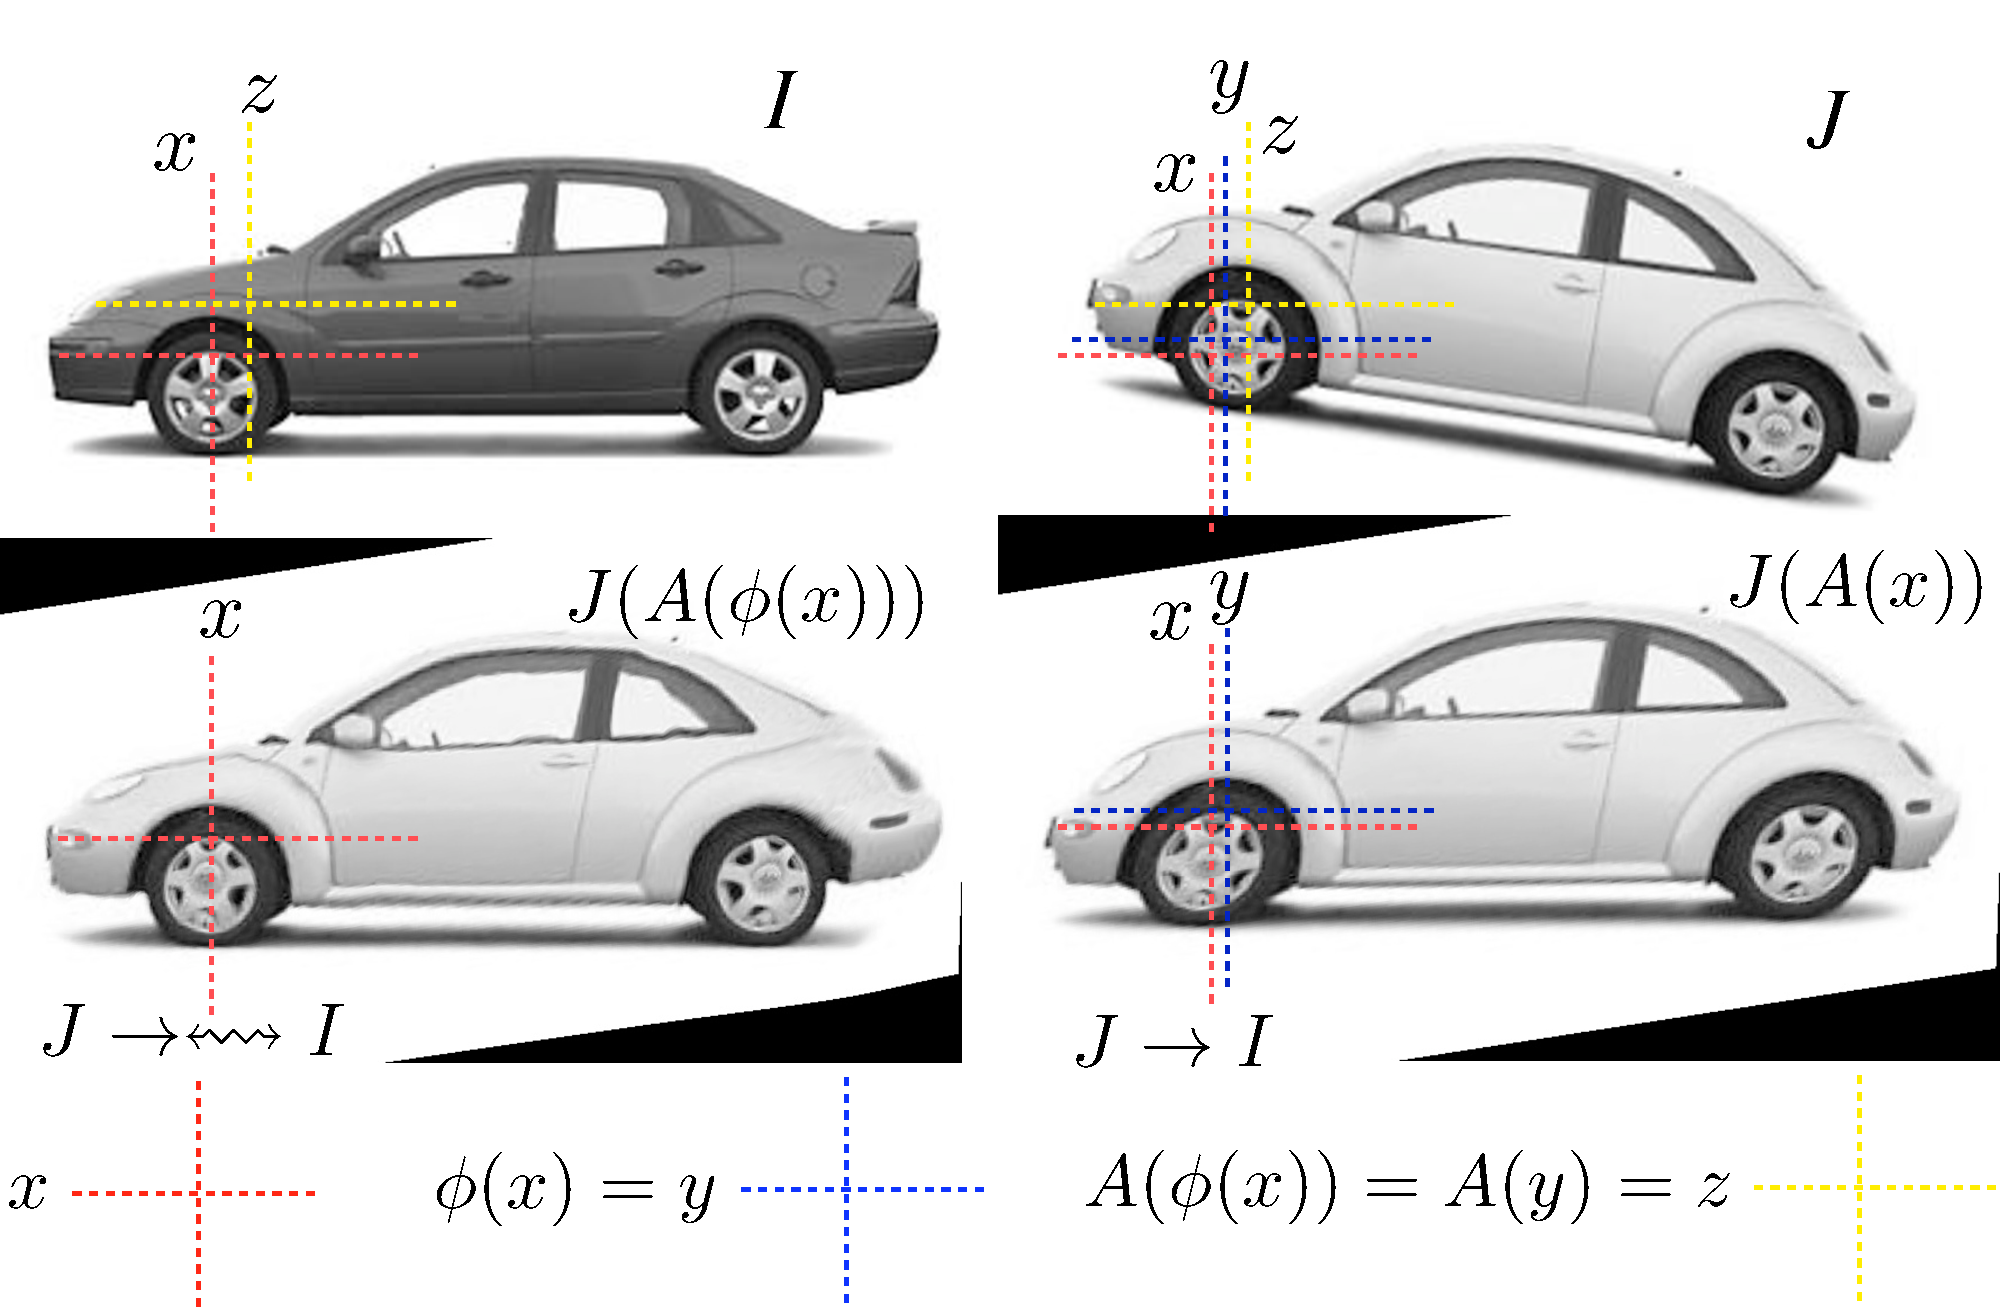
\includegraphics[width=5in]{figs/RegistrationNomenclature.pdf}
\end{tabular}
\caption{Clockwise:  Define $x$ in $\Omega_I$ and $z$ in
  $\Omega_J$ as the same material point but existing in different
  domains.  The point $y$ is in a domain that is intermediate between
  $\Omega_I$ and $\Omega_J$.  The standard approach in the ITKv4
  registration framework is to map image $J$ (b) to image $I$ (a) by first
  identifying the linear transformation, $\rightarrow$, between the images, shown in (c).  Second, we remove the shape (diffeomorphic)
  differences (d).  Consequently, we have a composite mapping, computed via the
  mutual information similarity metric, that identifies
  $I(x) ~\approx_\text{mi}  J(A(\phi(x))) =  J_\text{Affine}(y) = J(z)
  $. The image $J_\text{Affine}(y)$
  represents $J$ after application of the affine transformation $A$
  i.e., $J(A(x))$.  Code and data for this example are
  \href{http://stnava.github.io/cars/}{here}.  }
%  We avoid compounding interpolation  error by concatenating transformations.  Thus, we never need to use more than  a single interpolation into the data regardless of the nature of the  sub-transforms within the composite mapping.  Because transformations may  either perform mapping or resampling, this framework also  provides the ability to handle changes in resolution.}
\label{fig:composite}
\end{center}
\end{figure}

Finally, we summarize \tk changes through quantitative metrics:
\begin{itemize}
\item~Over 12 new multi-threaded image registration metrics are available in v4.
\item~Four application-level registration methods, with plug-and-play architecture, are available
  for high-level inclusion in projects such as Slicer and SimpleITK.
\item~All contributions are unit-tested and have greater than 85\% code coverage, in accordance with ITK standards.
\item~A complete refactoring of the ITK transform hierarchy that makes transforms thread-safe, applicable to high-dimensional optimization and easily used in multi-core computing. 41 classes, in total, were impacted by this refactoring.
\item~We added transparent vector support to two key interpolators that are used
  pervasively in ITK: the nearest neighbor and linear interpolators.
  We added two new Gaussian interpolators.
\item~An example of vector support for image metrics is in \newline \texttt{itkMeanSquaresImageToImageMetricv4VectorRegistrationTest.cxx}.
\end{itemize}
Below we will discuss: (0) an organizing nomenclature matched to the
\tk framework, (1) gradient-based optimization within the
framework, (2) techniques to estimate optimization parameters for
arbitrary metric and transformation combinations, (3) a \tk instance implementing generalized diffeomorphic
matching, (4) several
applications of the updated framework within different
neuroinformatics-relevant domains.

\subsection{Nomenclature}
The nomenclature below designates an image registration
algorithm symbolically.  This nomenclature is intended to be a
descriptive and technically consistent system for visually
representing algorithms and applications of registration.  Ideally,
any standard algorithm can be written in the nomenclature below.
\newline
\noindent\makebox[\linewidth]{\rule{\textwidth}{0.4pt}}
\newline
\noindent\textit{begin nomenclature definition}
\vspace{0.1in}
\begin{Parallel}[c]{0.24\textwidth}{0.74\textwidth}
\ParallelLText{A physical point:} \ParallelRText{\noindent $x \in \Omega$ where $\Omega$ is the domain,
  usually of an image.}\vspace{0.075in}
\ParallelPar
\ParallelLText{An image:} \ParallelRText{\noindent $ I \colon \Omega^d \to \mathbb{R}^n$ where $n$ is the
  number of components per pixel and $d$ is dimensionality.  A second
  image is $J$.}\vspace{0.075in}
\ParallelPar
\ParallelLText{Domain map:} \ParallelRText{\noindent $ \phi \colon \Omega_I \to \Omega_J $ where $\to$ may be
  replaced with any mapping symbol below.} \vspace{0.075in}
\ParallelPar
\ParallelLText{Affine mapping:} \ParallelRText{\noindent $\leftrightarrow$ a low-dimensional invertible 
  transformation: affine, rigid, translation, etc.} \vspace{0.075in}
\ParallelPar
\ParallelLText{Affine mapping:} \ParallelRText{\noindent $\rightarrow$ designates the direction an
  affine mapping is applied.}\vspace{0.075in}
\ParallelPar
\ParallelLText{Deformation field:} \ParallelRText{\noindent  $ \rightsquigarrow$ deformation field mapping $J$
  to $I$.  May not be invertible.}\vspace{0.075in}
\ParallelPar
\ParallelLText{Spline-based mapping:} \ParallelRText{\noindent  $\substack{
   \rightsquigarrow \\
   b
  }$ e.g., B-Spline field mapping $J$
  to $I$.}\vspace{0.075in}
\ParallelPar
\ParallelLText{Diffeomorphism:} \ParallelRText{\noindent Represented
  as $\leftrightsquigarrow$, these are differentiable maps with
  differentiable inverse.  Ideally, the algorithm should output the
  inverse and forward mapping.}\vspace{0.075in}
\ParallelPar
\ParallelLText{Composite mapping:} \ParallelRText{\noindent $\phi=\phi_1(\phi_2(x))$ is defined by
  $ \leftrightsquigarrow \rightarrow $ where $\phi_2$ is of type
  $\leftrightsquigarrow$.}\vspace{0.075in}
\ParallelPar
\ParallelLText{Not invertible:} \ParallelRText{\noindent $\nleftrightarrow$ indicates a mapping that is
  not invertible.}\vspace{0.075in}
\ParallelPar
\ParallelLText{Perform image warping:} \ParallelRText{\noindent As an example, $ \rightarrow J$ represents
the application of an affine transform $\rightarrow$ to image $J$ such that
$\rightarrow J = J( A( x ) ) $.}\vspace{0.075in}
\ParallelPar\vspace{0.075in}
\ParallelLText{Similarity measure:}\ParallelRText{\noindent $\substack{
   \approx \\
   s
  }$ or $\approx_s$ indicates the metric $s$ that compares a pair of images.}
% \item [Transport versus diffeomorphism] intrasubject versus intersubject.
% \item [Resolution effects]  ...
% \item [accuracy vs precision] obsessed with accuracy because we dont
% know the precision we need
% \item [Evaluation data] is there any?
% \item [Serial vs longitudinal]  short time scale versus long time scale
% \item [Pathology] appearance changes ...
% \item [whole body atlas] map any image to whole body
% \item [radiation oncology] techs understand translation versus rotation versus deformation.
\end{Parallel}
\vspace{0.1in}
\noindent\textit{end nomenclature definition}\newline
\noindent\makebox[\linewidth]{\rule{\textwidth}{0.4pt}}
\newline

We would then write a standard Demons registration application that maps 
one image, $J$, into the space of $I$ (presumably a template) as:
$$
 I  \rightsquigarrow \rightarrow  J \text{~~~~~which symbolizes~~~~~} I \approx
 J( A( \phi( x ) )),
$$
with $A$ an affine mapping and $\phi$ a generic deformation. 
The notation means that the algorithm first optimizes an affine
mapping, $ \rightarrow$, 
between $J$ and $I$.  
This is followed by a deformation in the second stage,$\rightsquigarrow$, from $\rightarrow J$
to $I$.  In terms of transformation composition, we would write
$\rightsquigarrow \rightarrow  J = J_w(x) =
J( \phi_\text{Affine} ( \phi_\text{Demons} ( x) )) $ where $J_w$ is
the result of warping $J$ to $I$.  The $\phi$ are the specific
functions corresponding to the schematic arrows.  Note, also, that the
tail of the arrow indicates the transform's domain.  The arrowhead
indicates its range.  Finally, we denote the similarity metric as
$\approx$ which indicates a sum of squared differences (the default
similarity metric).  \tk supports metrics such as mutual information,
$\substack{ \approx \\ \text{mi} }$, or cross-correlation, $\substack{
\approx \\ \text{cc} }$.  We will use this nomenclature to write
schematics for registration applications in the following sections.
\footnote{In the Demons example above, the reader may ask: why does the affine
mapping, $A$, not appear ``inside'' the deformable mapping, $\phi$?
Indeed, this ordering of transformations is feasible.  However, this is not
what we typically use in our own practice of image registration and is
not what we recommend.  The
reason is that we usually seek a deformable mapping into a template
space that is common across many subjects (i.e., the ``tail'' is in the
same domain across subjects).  This enables methods such as
Jacobian-based morphometry and other groupwise comparison
conveniences.  For example, see Figures 1 through 4 in \cite{Kim2008}
which explains the classical approach of Jacobian-based morphometry as
applied to traumatic brain injury.  See also
\cite{Studholme2007,Lepore2006,Rohlfing2006,Dubb2005,Riddle2004,Gaser2001}.
Additional uses of Jacobian-based morphometry are shown in our examples section in the
``C'' example and the ``asymmetry'' example.}


\subsection{Optimization Framework}
The general \tk optimization criterion is summarized as:
\begin{eqnarray}
\text{Find mapping}~\phi(x,p) \in \mathcal{T}
\text{such that}~M(I,J,\phi(x,p))~\text{is minimized}. 
\label{eq:gen}
\end{eqnarray}
While, for functional mappings, this formulation is not strictly correct, the
practical implementation of even high-dimensional continuous
transformations involves parameterization. 
The space $\mathcal{T}$ restricts the possible transformations over
which to optimize the mapping $\phi$.  The arguments to $\phi$ are its
parameters, $p$, and the spatial position, $x$.  Note that, in \tk,
the image $I$ may also contain a mapping, although it is not directly
optimized in most cases.  As will be seen later in the document, this
mapping may also be used within large deformation metrics. 

The similarity metric, $M$, is perhaps the most critical component in image registration.  
Denote a parameter set as $p = (p_1, p_2 \ldots p_n)$.  
The metric (or comparison function between images) is then defined by $M(I,J,\phi(x,p))$.  For instance, $M=\|
I(x)-J(\phi(x,p)) \|^2$ i.e., the sum of squared differences (SSD) metric. Its gradient with respect to parameter $p_i$
is (using the chain rule), 
\begin{eqnarray}
 M_{p_i}=\frac{\partial M}{\partial
  p_i}=\frac{\partial M}{\partial J}\frac{\partial
  J(\phi(x,p))}{\partial \phi} \frac{\partial \phi}{\partial p_i}^T|_x
~~.
\label{eq:grad}
\end{eqnarray}
This equation provides the metric gradient specified for
sum of squared differences (at point $x$) but similar forms arise for the correlation
and mutual information \citep{hermosillo}.  Both are implemented in
\tk for transformations with local and global support.  The
$\frac{\partial J(\phi(x,p))}{\partial \phi}$ term is the gradient of $J$ at $\phi(x)$
and $\frac{\partial \phi}{\partial p_i}$ is the Jacobian of the transformation taken
with respect to its parameter.   The transform $\phi(x,p)$ may be
an affine map i.e., $\phi(x,p)=A x + t$ where $A$ is a matrix and
$t$ a translation.  Alternatively, it may be a displacement field
where $\phi(x,p)=x+u(x)$ and
$u$ is a vector field.  In \tk, both types of maps are interchangeable
and may be used in a composite transform to compute registrations that
map to a template via a schematic such as $ I \approx \rightarrow J $, $ I $ ~\mi~\bsp~$
\rightarrow  J $, $ I $~\cc~$ \leftrightsquigarrow \rightarrow J $
or, mixing similarity metrics, $I
~\approx_\text{cc}  \leftrightsquigarrow \approx_\text{mi}  \rightarrow
J_i $.  

The most commonly used optimization algorithm for image registration
is gradient descent, or some variant.   In the above framework, the
gradient descent takes on the form of
$$
\phi(p_\text{new},x)=\phi\left(p_\text{old}+\lambda~\left[ \frac{\partial
  M}{\partial p_1} , \cdots , \frac{\partial
  M}{\partial p_n} \right] ,  x \right),
$$
where $\lambda$ is the overall learning rate and the brackets hold the
vector of parameter updates.  

In addition to basic gradient descent, we implement nonlinear gradient
descent optimization strategies which combine the conjugate gradient
or gradient descent method with line search.  In ITK$^4$, we implement the classic \textit{golden section} approach to identifying the optimal gradient
step-size at each iteration.  The generic conjugate gradient approach
is performed via: 
\begin{align}
\gamma=\frac{\|\nabla M_{t}-\|\nabla M_{t-1}\|^2\|^2}{\|\nabla
  M_{t-1}\|^2}, \\ \notag
CG_t = \nabla M_t + \gamma CG_{t-1},
\end{align}
where $CG$ is the conjugate gradient.  The golden section line search
determines the specific weight, $\epsilon_\text{opt}$, of the update to the current parameters
such that 
$$ 
p_{\text{new}}=p_{\text{old}}+CG_t \epsilon_\text{opt}.
$$
Note that a naive application of gradient descent will not produce a smooth
change of parameters for transformations with mixed parameter types.
For instance, a change, $\Delta$, to parameter $p_i$ will produce a
different magnitude of impact on $\phi$ if $p_i$ is a translation rather than a
rotation.  Thus, we develop an estimation framework that sets
``parameter scales'' (in ITK parlance) which, essentially, customize
the learning rate for each parameter.  The update to
$\phi$ via its gradient may also include other steps (such as Gaussian
smoothing) that project the updated transform back to space
$\mathcal{T}$.  Multi-threading is achieved in the gradient computation, transformation update
step and (if used) the regularization by dividing the parameter set
into computational units that correspond to contiguous sub-regions of the image domain.

In terms of code, the Jacobian, $\frac{d\phi}{dp}|_x$, is calculated at a physical point
using the function \textit{ComputeJacobianWithRespectToParameters(mappedFixedPoint, Jacobian)}.  
Note that it is evaluated at point $x$ not at point $\phi(x,p)$.  We
then use the function \textit{ComputeMovingImageGradientAtPoint(mappedMovingPoint,
mappedMovingImageGradient)} to compute the moving image gradient
when there is no pre-warping.  \textit{ComputeMovingImageGradientAtPoint} uses central
differences (or a gradient filter) in the moving image space to
compute the image gradient, $\frac{dJ(\phi(x,p))}{d\phi}$.

 If one is doing pre-warping, then we have an index access to the
 warped moving image.  We compute the warped image $J$ as
 $J_w(x)=J(\phi(x,p))$.  Then,
\begin{eqnarray}
\frac{dJ_w}{dx}=\frac{dJ(\phi(x,p))}{d\phi}\frac{d(\phi(x,p))}{dx} \\ \notag
\frac{dJ(\phi(x,p))}{d\phi}=\frac{dJ_w}{dx}{\frac{d(\phi(x,p))}{dx}}^{-1}.
\end{eqnarray}
In code, we use \textit{ComputeMovingImageGradientAtIndex(index,
mappedMovingImageGradient)} to get $\frac{dJ_w}{dx}$ and transform
this image gradient via the inverse Jacobian by calling 
\textit{mappedMovingImageGradient=
TransformCovariantVector(mappedMovingImageGradient, mappedMovingPoint)}.


\subsection{Diffeomorphic mapping with arbitrary metrics}
\begin{figure}[t]
\begin{center}
\begin{tabular}{c}
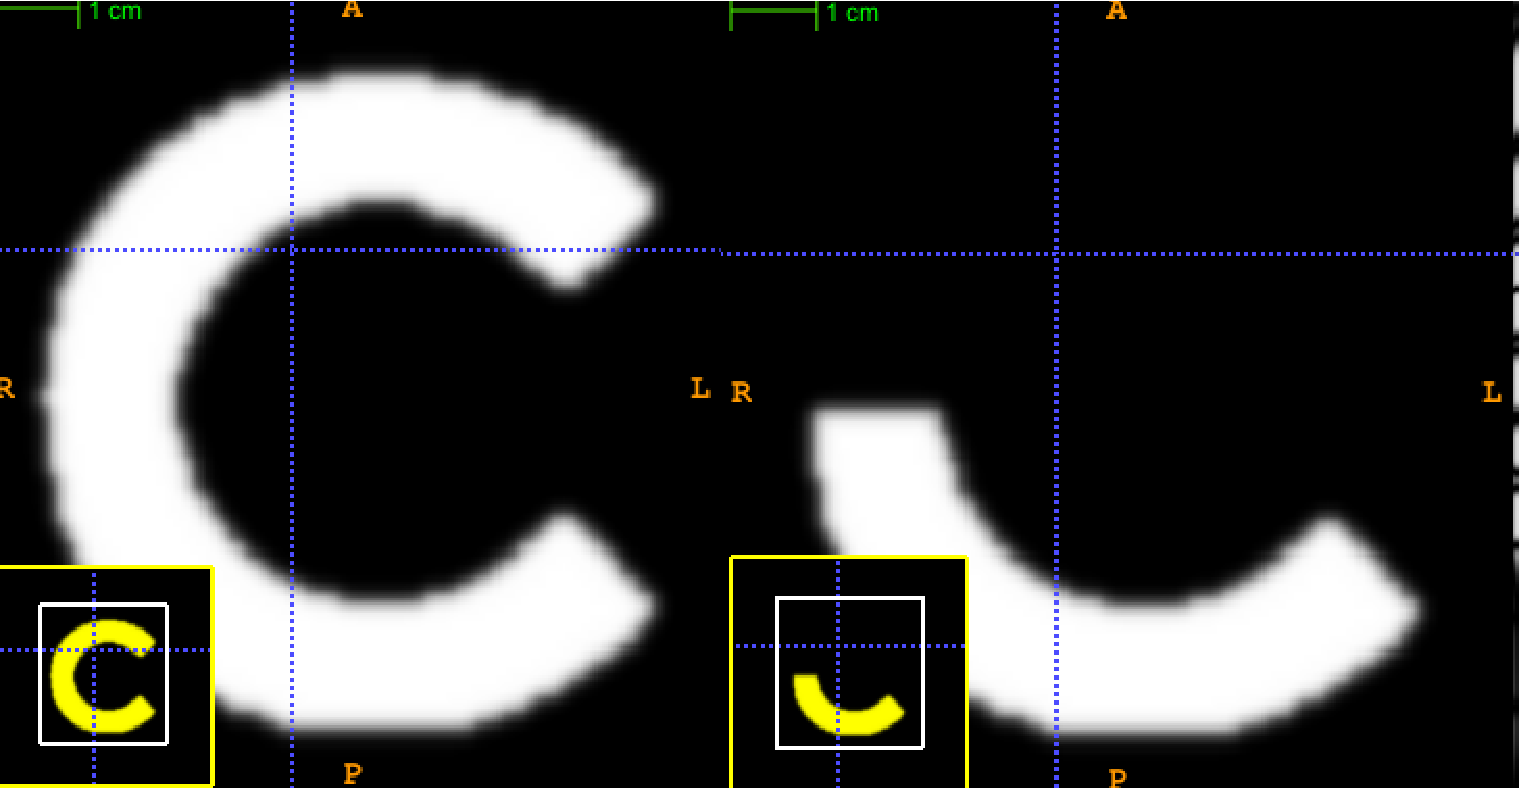
\includegraphics[height=1.6in]{figs/c_chalf.pdf}
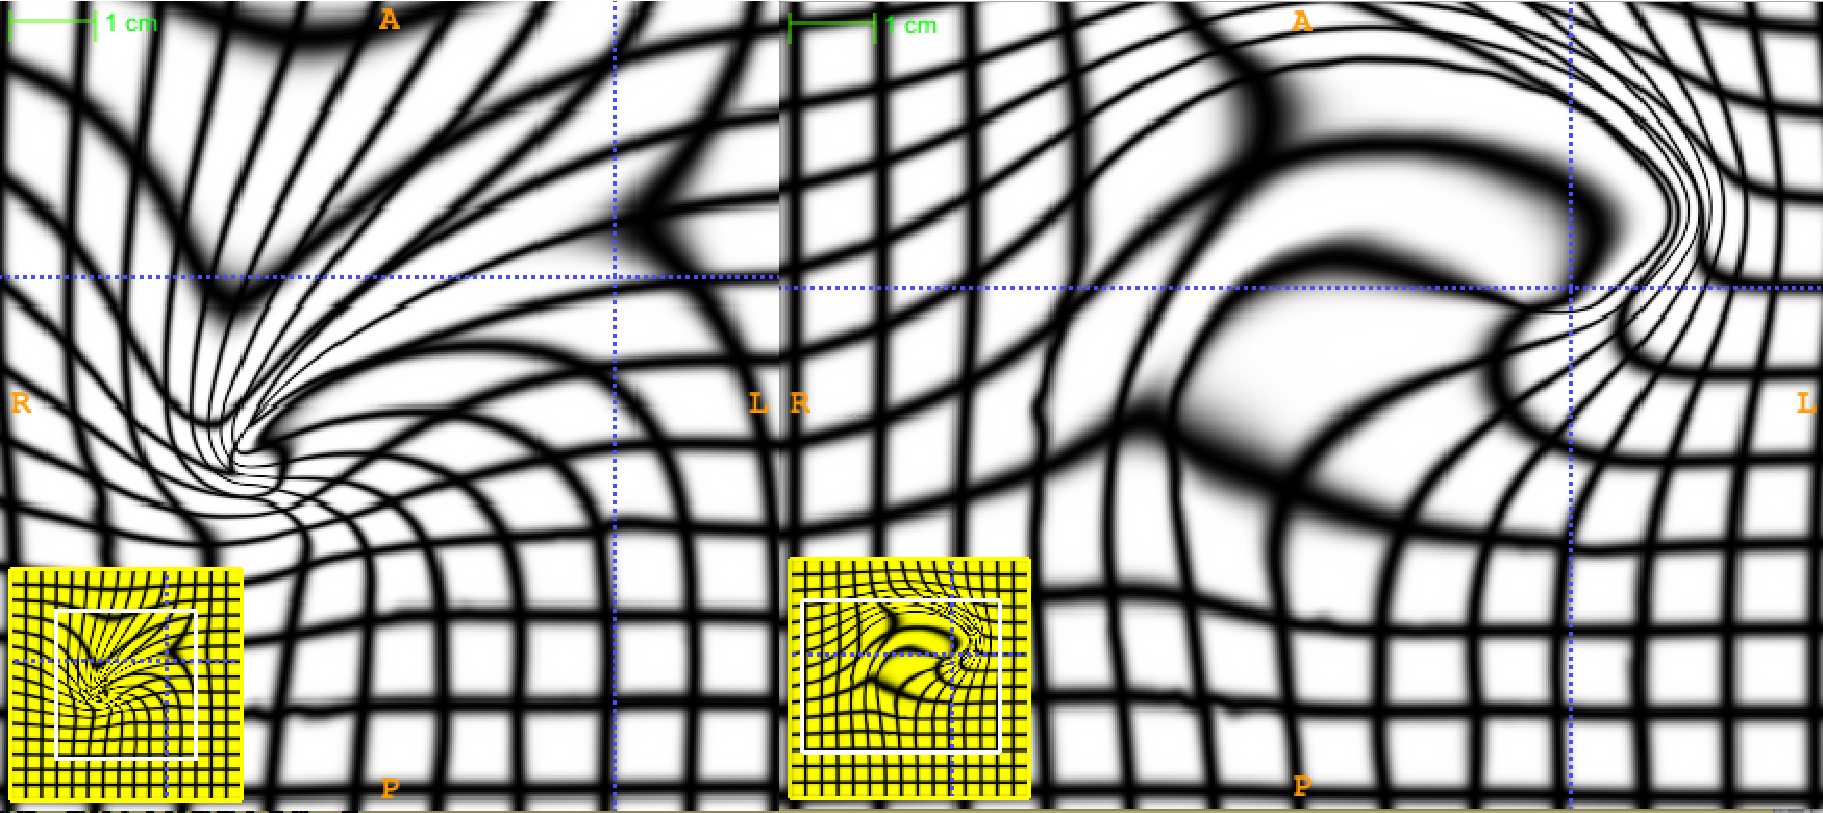
\includegraphics[height=1.6in]{figs/c_half_c_grids.pdf}
\end{tabular}
\caption{An ITK diffeomorphic mapping of the
  type $I \leftrightsquigarrow J $.  The 
``C'' and 1/2 ``C'' example illustrate the large deformations that may
be achieved with time varying velocity fields.  In this case, the moving (deforming) image is
the 1/2 ``C''.  The right panels illustrate the deformed grid for the
transformation of the ``C'' to 1/2 ``C'' (middle right) and its
inverse mapping (far right) which takes the 1/2 ``C'' to the reference
space.  The unit time interval is discretized into 15 segments in
order to compute this mapping.  15*5 integration steps were used in
the Runge-Kutta ODE integration over the velocity field.  A two
core MacBook Air computed this registration in 110 seconds.  The images
each were of size $150 \times 150$.  See
\href{http://stnava.github.io/C/}{C} for a reproducible example of
this registration and the data.  In addition, we provide an example of
how the Jacobian determinant is computed from the deformation field
resulting from this registration via an \textit{ANTs}
program \texttt{CreateJacobianDeterminantImage}.}
\label{fig:chalf}
\end{center}
\end{figure}

The framework proposed above, in general form, encompasses both
classic affine mapping as well as more recent large deformation
strategies.  Beg proposed the Large Deformation Diffeomorphic Metric Mapping
(LDDMM) algorithm \citep{Miller2005} which minimizes the sum of squared differences
criterion between two images.  LDDMM parameterizes a
diffeomorphism through a time varying velocity field that is
integrated through an ODE.  In \tk, we implement an alternative
to LDDMM that also uses a time varying field and an ODE but minimizes
a more general objective function:
\begin{align}
\myE(\v) = M(I,J,\myphi_{1,0})
+  w \int_{0}^{1} \| \opL v_t\|^2 \dd t \;.
\label{eq:lddmm}
\end{align}
This is an instance of Equation~(\ref{eq:gen}) where $w$ is a scalar
weight and $\myphi_{1,0}$ is a standard integration of the
time-varying velocity field, $v_t$, which is regularized by the linear
operator $\opL$.  \tk uses Gaussian smoothing which is the Green's
kernel for generalized Tikhonov regularization \citep{Nielsen1997}.
This objective is readily optimized using an approach that is similar
to that proposed by Beg.  Generalization of the LDDMM gradient 
for other metrics basically follows \citep{hermosillo} with a few
adjustments to accomodate diffeomorphic mapping.
Figure~\ref{fig:chalf} shows an ITK result on a standard example for
large deformation registration.  We will evaluate this diffeomorphic
mapping, along with parameter estimation, in a later section.

\subsection{Parameter scale estimation}
We choose to estimate parameter scales by analyzing the result of a
small parameter update on the change in the magnitude of physical space deformation
induced by the transformation.  The impact from a unit change of
parameter $p_i$ may be defined in multiple ways, such as the maximum shift of
voxels or the average norm of transform Jacobians \citep{Jenkinson2001}.
Denote the unscaled gradient descent update to $p$ as $\Delta
p$.  The goal is to rescale $\Delta p$ to $q = s \cdot \Delta p$, where $s$ is a diagonal
matrix $\text{diag} (s_1, s_2 \ldots s_n)$, such that a unit change of $q_i$ will have
the same impact on deformation for each parameter $i = 1\ldots n$.   

As an example, we want $ \| \phi(x,p_{\text{new}}) -
\phi(x,p_\text{old}) \| = constant $ regardless of which of the
$i$ parameters is updated by the unit change.  The unit is an epsilon
value e.g., 1.e-3.
Rewrite $\left[ \frac{\partial
  M}{\partial p_1} , \cdots , \frac{\partial
  M}{\partial p_n} 
 \right]$ as $\frac{\partial M}{\partial J}\frac{\partial
  J(\phi(x,p))}{\partial \phi} \left[ \frac{\partial \phi}{\partial p_1} , \cdots , \frac{\partial \phi}{\partial p_n} \right]$.
To determine the relative scale effects of each parameter, $p_i$, we
can factor out the constant terms on the outside of the bracket.  
Then the modified gradient descent step becomes
$\text{diag}(s)\frac{\partial \phi}{\partial p}$.  We identify the values
of $\text{diag}(s)$ by explicitly computing the values of $\| \phi(x,p_{\text{new}}) -
\phi(x,p_\text{old}) \| $ with respect to an $\epsilon$ change.  A critical variable,
practically, is which $x$ to choose for evaluation of $\| \phi(x,p_{\text{new}}) -
\phi(x,p_\text{old}) \| $.  The corners of the image domain work well
for affine transformations.  In contrast, local regions of small radius
(approximately 5) work well for transformations with local support.
Additional work is needed to verify optimal parameters for this new
\tk feature.  However, a preliminary evaluation is performed in the results
section.  The new parameter scale estimation effectively reduces the number of parameters
that the user must tune from $k+1$ ($\lambda$ plus the scales for each
parameter type where there are $k$ types) to only 1, the learning
rate.  

The learning rate, itself, may not be intuitive for a user to set.
The difficulty---across problem sets---is that a good learning rate for
one problem may result in a different amount of change per iteration
in another problem.  Furthermore, the discrete image gradient may
become invalid beyond one voxel.  Thus, it is good practice to limit a 
deformation step to one voxel spacing
\citep{Jenkinson2001}.  We therefore provide the users the ability to
specify the learning rate in terms of the \textit{maximum physical space change
  per iteration}.  As with the parameter scale estimation, the domain
over which this maximum change is estimated impacts the outcome and
similar practices are recommended for both cases.   This feature is
especially useful for allowing one to tune gradient descent parameters
without being concerned about which similarity metric is being used.
That is, it effectively rescales the term $\lambda \partial M / \partial p$ to
have a consistent effect, for a given $\lambda$, regardless of the
metric choice.  In combination with our nonlinear conjugate gradient
approach (our current optimization of choice for linear registration),
this strategy drastically reduces the parameter setting burden for
users. 

\section{Results}
\subsection{Example Applications of the ITK$^4$ Framework}
\label{sec:applications}
As part of our work in ITK refactoring, we built, in parallel to
library programming, an
application interface that allows high-level access to the deep layers
of ITK registration.  These currently exist in the \textit{Advanced
  Normalization Tools} (ANTs) software
\href{http://stnava.github.io/ANTs}{(link)}.  While ANTs still serves
as intermediate (vs. direct) access-point to these tools, it provides
a high-degree of customization possibilities simply through a command
line interface and scripting.  Therefore a user is not required to
write new low-level (interestingly, C++ is now considered ``low-level'') software.  

Despite its relative youth, the ANTs wrapping of ITK functionality has
been employed with notable success in recent public, unbiased,
international evaluation studies.   ANTs was instrumental to a
first-place finish in SATA 2013 in two of three categories (based on
the median performance) where the ANTs approach was considerably
simpler than that employed by close finishers.  While the evaluation
of deep-gray matter registration showed relatively subtle differences,
the ANTs solution to the multivariate
canine leg data outclassed all other entrants.  Notably, the ANTs
solution used a multiple metric approach that simultaneously compared
two modalities during registration as in \cite{Avants2008}.  In the
cardiac data, the ANTs solution was the only one that was fully
automated resulting in a $\approx$15\% performance loss which can easily be
overcome by a modicum of user intervention.   Furthermore, ANTs/ITK-based
methods finished a clear first-place in the BRATS 2013 challenge.  Our entry
used intensity asymmetry as a key feature to segment brain tumors based
on multiple modality MRI.  Thus, these methods are within the leading
ranks of image registration methodologies as evaluated in recent work
as well as in the more traditional brain \citep{Klein2010} and lung CT
\citep{Murphy2011} studies. 

The ANTs contribution is valuable, in part, because of the tremendous range of
registration problems that exist in neuroinformatics and biomedical
imaging in general.  While it is not possible to solve all registration problems with a
general framework, one cannot afford to invent new
solutions for every instance one encounters.  Our general optimization-driven strategies have
proven to be invaluable to setting performance standards in a variety
of application domains.   In this section, we highlight some of the
lesser known capabilities of ANTs and ITK$^4$ with reproducible
examples that include data and specific commands to ANTs and/or ITK.  
A list of these examples follows:
\begin{enumerate}
  \item~The \href{http://stnava.github.io/BasicBrainMapping/}{Basic
      Brain Mapping} example shows how one can map two ``whole head''
    T1-weighted MRIs where one is a template that contains a researcher's prior
    knowledge defining the ``interesting'' parts of the image.  Within
    \tk, this domain knowledge is used to focus the \texttt{Metricsv4}
    on only those parts of the image while masking the remainder.
    Furthermore, a second part of this example shows how the ITK
    composite transform may be used to initialize new registration
    solutions as well as how masking functionality may be employed to
    ignore information that is irrelevant or obstructive to the
    registration optimization.  We have previously employed these
    strategies in brain mapping with lesions \citep{Avants2008,Kim2008,Kim2010,Tustison2011a,Kim2013}. 
  \item~We use updated ITK methods in template construction with a
    reproducible example based on face and brain data:
    \href{https://github.com/ntustison/TemplateBuildingExample}{ANTs
      template construction}.  This work has been employed in
    different species, age-ranges and imaging modalities.  The
    resulting template is an image that captures the expected shape
    and appearance as defined by the population sample, transformation
    model and intensity comparison metric.
  \item~A \href{http://stnava.github.io/C/}{large deformation
      example} implementing the classic ``letter C'' example provided,
     originally, by Gary Christensen.  While extremely flexible, these
     algorithms have not found a unique identity in terms of
     translational applications yet remain of theoretical interest.
     This example shows a user how to define the parameters of a
     registration based on optimizing a time
     varying velocity field.
  \item~We present a separate example of how to compute landmark-based
    registration error.  ITK uses LPS coordinates to represent physical space.  If you
    need to convert landmarks to physical space, see the discussion here:
    \href{http://sourceforge.net/p/advants/discussion/840261/thread/2a1e9307/}{LPS
      physical
      space}.  We have an example illustrating how to change point
    coordinates and apply ITK transforms to landmarks
    \href{http://stnava.github.io/chicken/}{here}.  This exercise can
    be useful for landmark-based registration or in evaluating
    registration accuracy.
  \item~We show how to perform motion correction to time series data
    \href{https://github.com/stnava/ANTs/blob/master/Scripts/antsMotionCorrExample}{here}
    although we do not claim this approach is optimal.  The method
    registers each frame from a 4D time series to a fixed reference
    image and stores the resampled set in a new 4D image.  All
    transformation parameters are stored in a corresponding csv file.
   \item~ An advanced example with heavy use of statistics via \textit{R} and \href{http://stnava.github.io/ANTsR/}{\textit{ANTsR}} is in
     a study of \href{http://stnava.github.io/RfMRI/}{public
       test-retest fmri data}.  This study is not published and may be
      subject to change.
  \item~The classic car example shown in ANTs talks is
    \href{http://stnava.github.io/cars/}{here}.  This illustrates the
    benefit of mutual information in deformably mapping wild-type
    images and highlights the fact that \tk applications exist outside
    of medical imaging.
  \item~A basic \href{http://stnava.github.io/butterfly/}{multistart example}.  A more advanced
    example for brain mapping with a template mask is available in
    \textit{antsCorticalThickness.sh}.  These optimization methods
    overcome local minima by running registration searches from a
    variety of starting points and greedily storing the best solution.
   \item~  This \href{http://stnava.github.io/asymmetry/}{asymmetry
       analysis} example uses the ``virtual domain'' feature to reduce
     bias caused by mapping an image asymmetrically to a reference.
     Note that we measure the point-wise asymmetry, in this example,
     via the Jacobian determinant image as in \cite{Kim2008}.  If one
     repeats this analysis across a population---and maps the Jacobian
     measurements of asymmetry to a common space---then one may perform a
     statistical analysis of population-level asymmetry.
     Longitudinal analysis and asymmetry analysis potentially suffer
     from the same confound \cite{Yushkevich2010a}.  A related
     longitudinal mapping script is \href{https://github.com/stnava/ANTs/blob/master/Scripts/unbiased_longitudinal_map}{here}.
  \item~We also show how manual labelings can be used to restrict
    registration in a challenging registration scenario (this example
    will be improved in the future): \href{http://stnava.github.io/LabelMyHeart/}{
    registration guided by (crude) labels}.  
 \item~A simple orange to apple RGB image registration example for
   color images is listed at:
   \href{https://github.com/Kitware/ITK/blob/master/Modules/Registration/Metricsv4/test/CMakeLists.txt}{itkMeanSquaresImageToImageMetricv4VectorRegistrationTest}.
   If one compiles the ITK tests, then this example can be run to
   produce Figure~\ref{fig:appleorange}.
\end{enumerate}
These examples cover many applications for which no ``ground truth''
evaluation data exists.  The next section seeks to add some
quantitative reference to these examples.  First, we show flexibility
and consistency of our framework in a simple example comparing
registration with a variety of metrics and a consistent parameter
set.  Second, we quantify the benefit of
\tk registration in comparison to a method implemented based upon \tkt
registration technology.
\begin{figure}[t]
\begin{center}
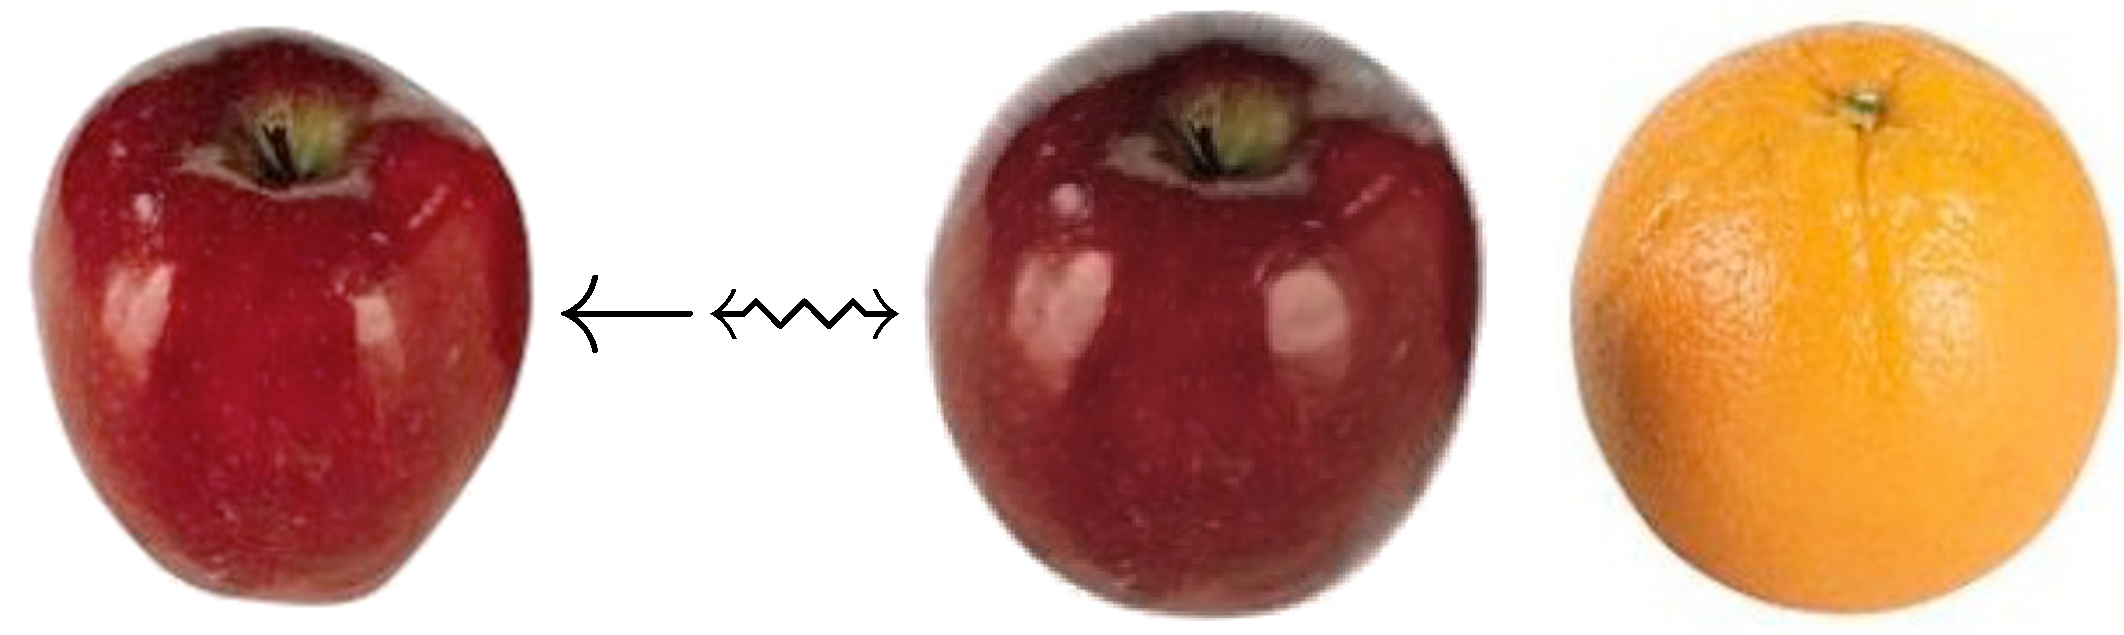
\includegraphics[width=6.5in]{figs/appleorange.pdf}
\caption{This RGB image registration example employs
  \tk code that repurposes a scalar metric
  (\texttt{itkMeanSquaresImageToImageMetricv4}) for
  multichannel registration.}
\label{fig:appleorange}
\end{center}
\end{figure}

\subsection{Evaluation}
We first investigate the ability of our automated parameter estimation
to facilitate parameter tuning across metrics.  Second, we compare
\tk and \tkt registration implementations with respect to a
standard automated brain labeling task.

\subsubsection{Parameter estimation across metrics}
\tk provides similarity metrics that may be applied for both
deformable and affine registration.  In a previous section, we
provided a parameter estimation strategy that is applicable to both
deformable and affine transformations with arbitrary metrics.  Denote
images $I$, $J$, $K$, where the latter two are ``moving'' images, and
$K$ is an intensity-inverted version of $J$.
We then evaluate the following schema,
\begin{eqnarray}
I \approx \leftrightsquigarrow  \rightarrow J,~~~~~~~
I \approx_\text{cc} \leftrightsquigarrow  \rightarrow  K,~~~~~~~  
I \approx_\text{mi} \leftrightsquigarrow  \rightarrow  K   \notag 
\end{eqnarray}
where, for each schematic, we use the corresponding metric for both
affine and diffeomorphic mapping.  Furthermore, we keep the same
parameters for each registration by exploiting parameter scale
estimators.  Figure~\ref{fig:result} shows the candidate images for
this test. 

As shown in Figure~\ref{fig:result}, very similar results are achieved
for each schematic without additional parameter tuning.  To determine
this quantitatively, we perform registration for each schematic and
then compare the Dice overlap of a ground-truth three-tissue
segmentation.  For each result, we have the Dice overlap of dark
tissue (cerebrospinal fluid, CSF), medium intensity tissue (gray
matter) and bright tissue (white matter).  For the mean squares
metric, we have: 0.588, 0.816 and 0.90; for CC, we have: 0.624, 0.786,
0.882; for MI, we have: 0.645, 0.779, 0.858.  Mutual information does
best for the CSF while mean squares does best for other tissues.  CC
performs in the mid-range for all classes of tissue.  Thus, a single
set of tuned parameters provides a reasonable result for an affine
plus diffeomorphic mapping across three different metrics.  While
improvement might be gained by further tuning for each metric, this
result shows that our parameter estimation method achieves the goal of
reducing user burden.
\begin{figure}[t]
\begin{center}
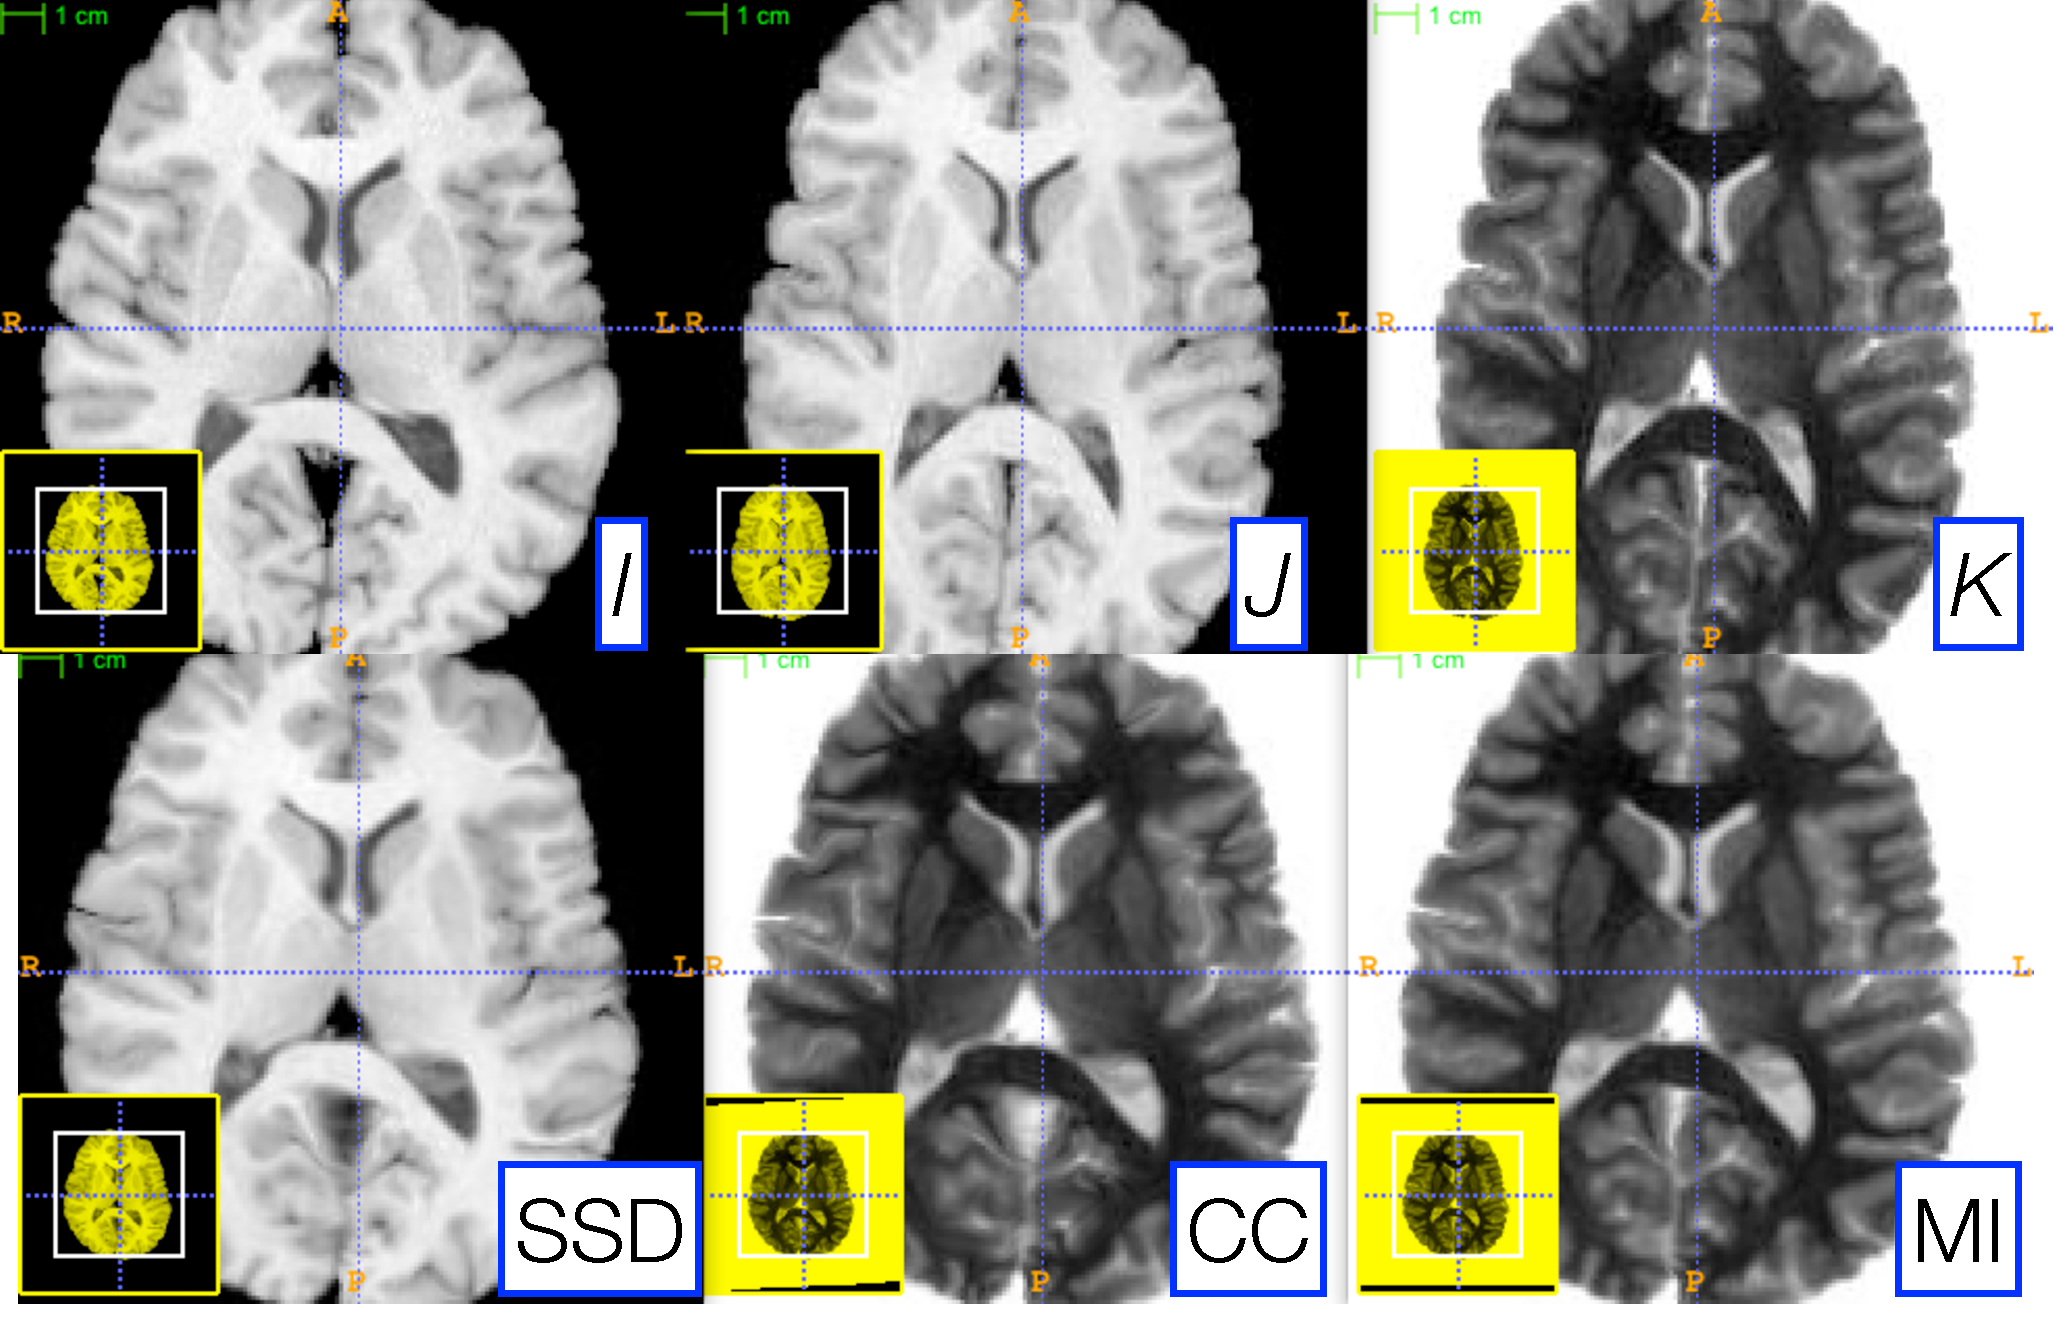
\includegraphics[width=4.5in]{figs/three.pdf}
\caption{Three reference images, $I$
(left), $J$ (middle top), and $K$ (right top), are used to illustrate
the robustness of our parameter scale estimation for setting
consistent parameters across both metrics and transform types.  $K$ is
the negation of $J$ and is used to test the correlation and mutual
information registrations.  We optimized, by hand, the step-length
parameters for one metric (the sum of squared differences) for both the affine
and deformable case.  Thus, two parameters had to be optimized.  We
then applied these same parameters to register $I$ and $K$ via both
correlation and mutual information.  The resulting registrations
(bottom row) were all of similar quality.  Further, the same metric is
used for both affine and diffeomorphic mapping by exploiting the
general optimization process given in Equation~(\ref{eq:gen}).}
\label{fig:result}
\end{center}
\end{figure}

\begin{figure}[t]
\begin{center}
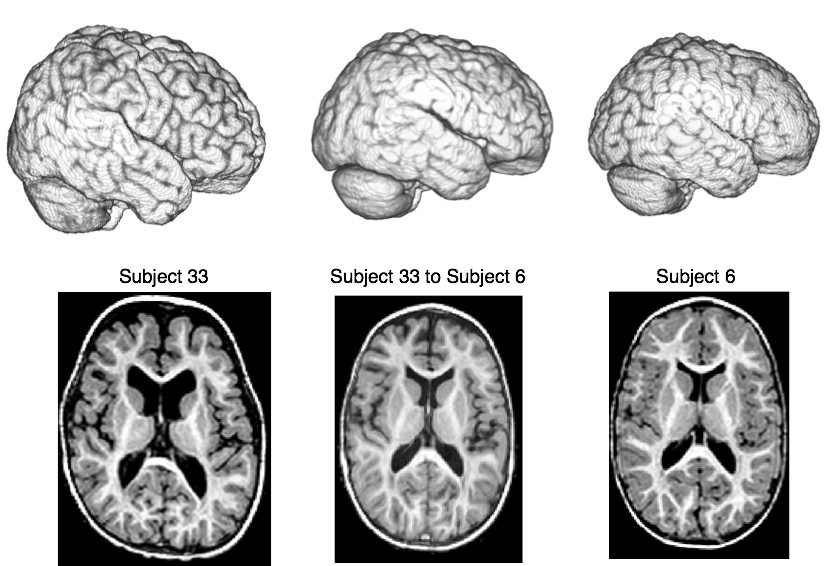
\includegraphics[width=5.5in]{figs/figEval.png}
\caption{We compare a \tk composite schema as $I
~\approx_\text{cc}  \leftrightsquigarrow \approx_\text{mi}  \rightarrow
J_i $ for mapping a set of $\{ J_i \}$ images
to a template $I$ to a \tkt schema:  $I
~\approx_\text{mi} \rightsquigarrow_b    \approx_\text{mi}  \rightarrow
J_i $.  We use this schematic in a registration-based
segmentation of multiple brain structures in a pediatric population as a benchmark
for algorithm performance, similar to \cite{Klein2010}.  An example ANTs-based
large-deformation result from the dataset is shown for illustration
where we render the extracted brains as well as show select axial
slices.  All registrations were run on the original MRI data with no
preprocessing except what is done by ANTs or BRAINSFit internally. Overlap improvement from v3 to v4, quantified via
paired t-test, is highly significant.}
\label{fig:eval}
\end{center}
\end{figure}

\subsubsection{Automated Brain Labeling Task}
All \textit{R} and bash analysis scripts for this section are here:
\href{https://github.com/stnava/ITKv4Documentation/tree/frontiers/scripts}{https://github.com/stnava/ITKv4Documentation/tree/frontiers/scripts}.
The \tk core functionality formed the heart of the reference results
provided for the SATA2013 challenge at MICCAI 2013.  In this sense,
these methods have been heavily evaluated on both basic brain mapping
challenges (SATA2013's diencephalon challenge in which \tk-based
methods finished first), multivariate
registration challenges (the canine MRI / dog leg challenge of
SATA2013 in which \tk-based methods were overwhelmingly the top
finisher) and in the cardiac challenge (in which \tk-based methods
were the only fully automated approach).  However, for completeness,
we provide an additional evaluation here which focuses on comparison
to a \tkt method, BRAINSFit, in a different dataset than previously
used to evaluate ANTs or \tk.

As ground truth, we use T1 MRI data from 33 two year old subjects as
described in \cite{Gousias2008} and available at
\href{http://www.brain-development.org}{http://www.brain-development.org}.
Each subject's brain is manually parcellated into 83 distinct regions
that include ventricles, cortical areas, white matter and deep gray
matter regions such as the amygdala, hippocampus and thalamus.  One
benefit of this data is that some of these anatomical regions are
relatively easy to align (the caudate) whereas others are relatively
difficult to align due to their small size (amygdala) or inconsistent
shape across subjects (the inferior frontal gyrus).  Thus, we
anticipate that performance gains due to new technology in \tk will be
most prominent in the more variable and challenging regions.
Figure~\ref{fig:eval} summarizes the study nomenclature and shows a single image pair selected from this
data along with the registration result given by \tk.
Figure~\ref{fig:antsbfit} summarizes these evaluation results.  
The scripts for running this study are available at
\href{https://github.com/stnava/ITKv4Documentation/tree/frontiers/scripts}{https://github.com/stnava/ITKv4Documentation/tree/frontiers/scripts}.
The git hashtag for the ANTs version used in this evaluation \href{https://github.com/stnava/ANTs}{https://github.com/stnava/ANTs}
is
ce8b5a7414ae9e389071d756c5f36ee6cecbcfd8.  The associated ITK tag is contained
within the ANTs repository.  
The git hashtag for the BRAINSFit version \href{https://github.com/BRAINSia/BRAINSTools}{https://github.com/BRAINSia/BRAINSTools} used in this evaluation is
ad7e114ab1c92bd800819b80e0548259398931c8.  Both programs were run on a
MacBook Pro running OS X 10.9 (13A3028) with a 2.6 GHz Intel Core i7 and 16GB of RAM.
\begin{figure}[t]
\begin{center}
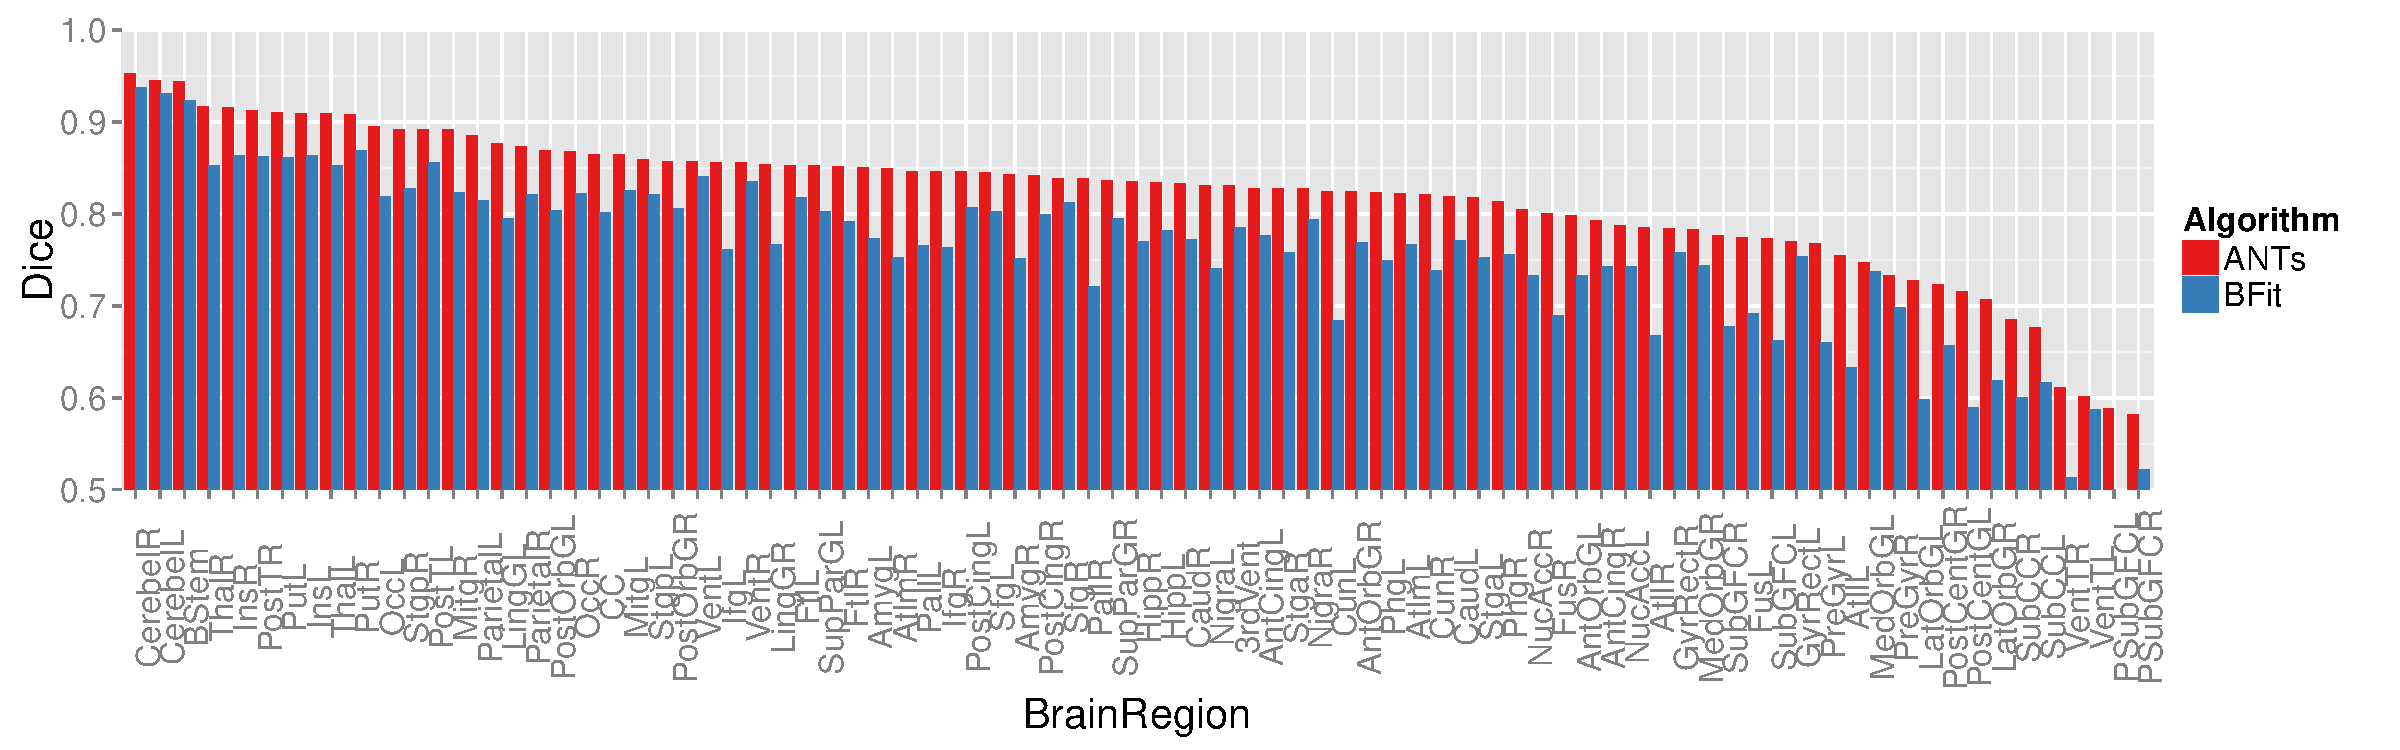
\includegraphics[width=6in]{figs/barplot.pdf}
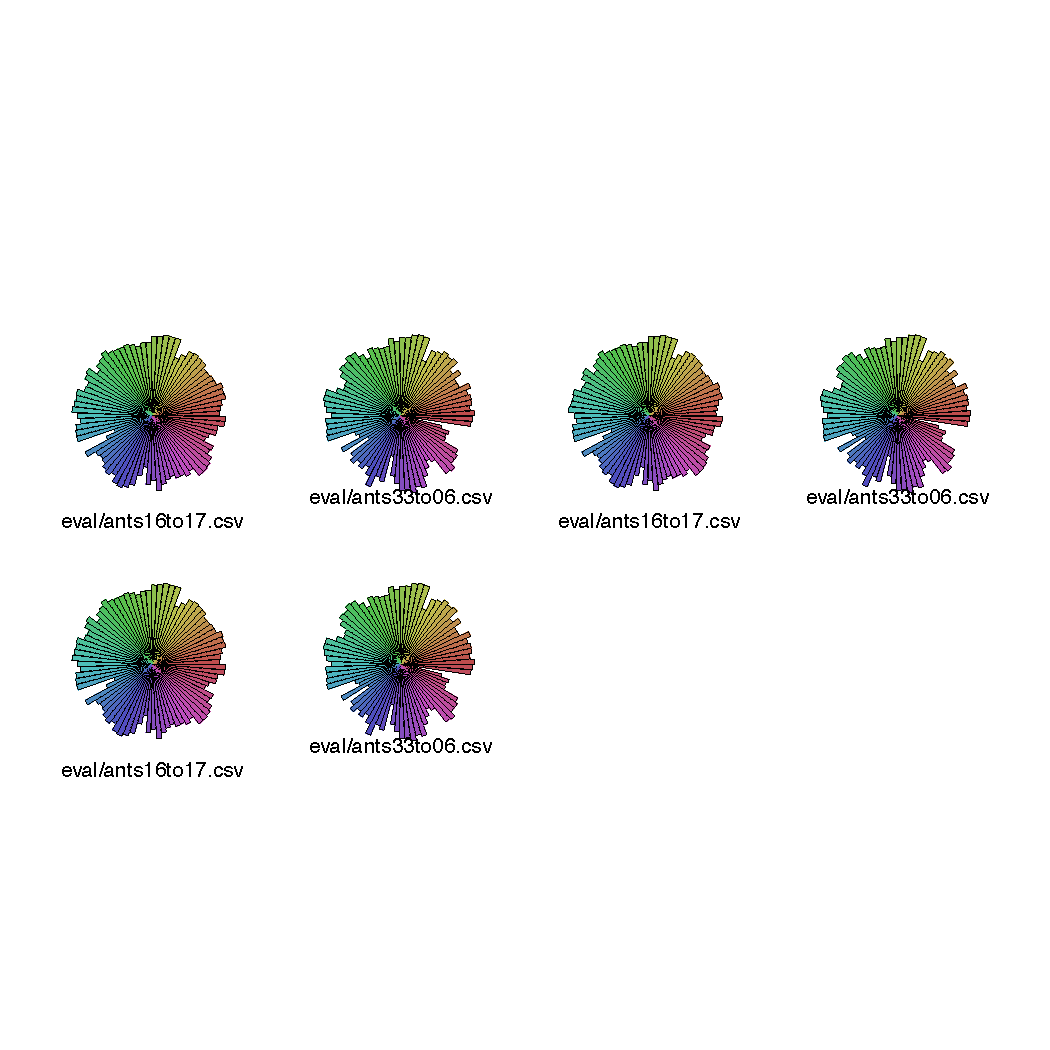
\includegraphics[width=6in]{figs/star_ants.pdf}
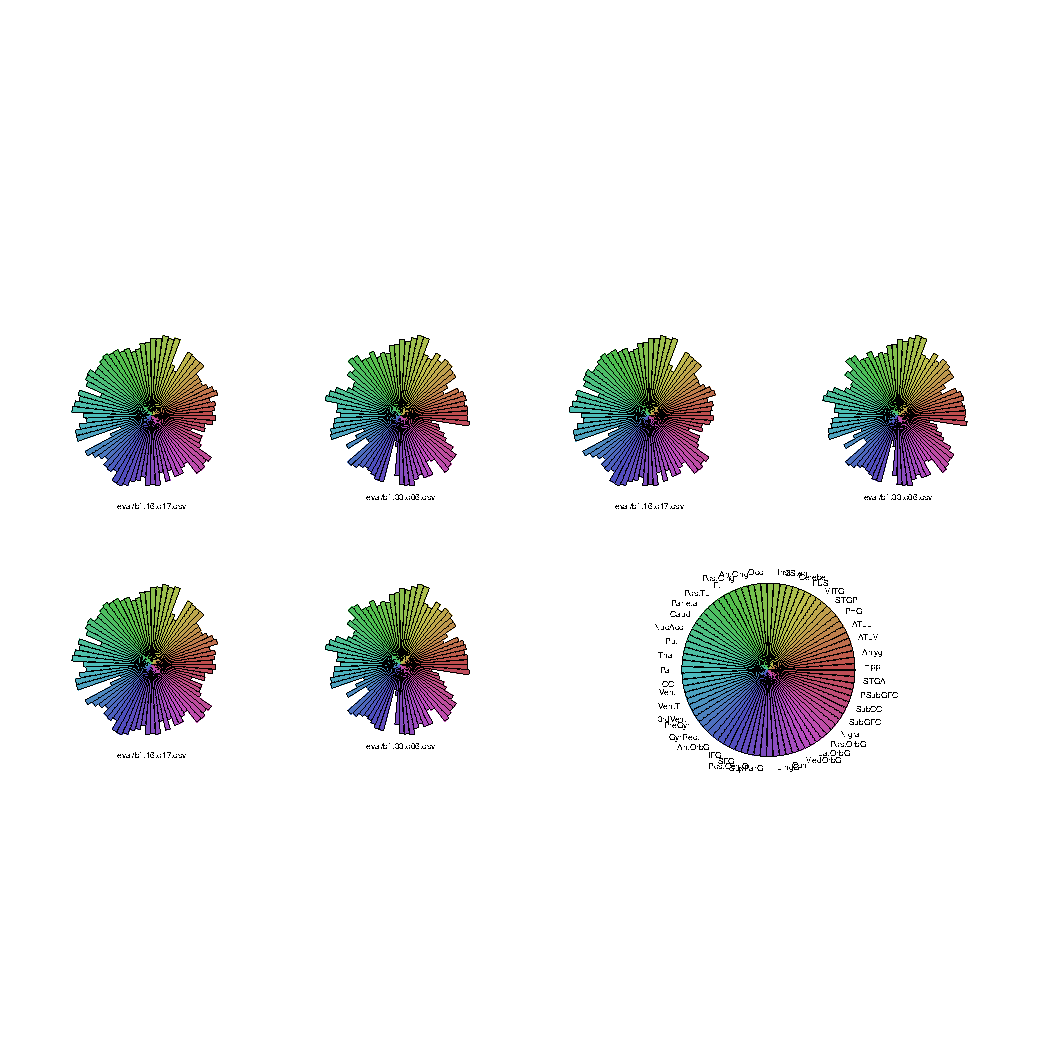
\includegraphics[width=6in]{figs/star_bfit.pdf}
\caption{Above, a barplot shows the mean Dice score for each region
  and each algorithm, sorted by ANTs performance.  Below, we use star plots of
  per-brain-region Dice overlap to compare, for each subject, the \tk
  implementation of SyN with the \tkt-based BRAINSFit algorithm.  The
  \tk SyN algorithm, with its classic neighborhood correlation
  metric, outperforms BRAINSFit in several regions and more strongly
  in some subject pairs than others.  The legend for the plots is at
  lower right and shows the maximum possible value for each region.}
\label{fig:antsbfit}
\end{center}
\end{figure}

To help isolate which subject pairs to deformably register, 
we first clustered the initial dataset based on an all pairs
affine registration which revealed five representative subject
clusters.   The subject pairings used during evaluation were chosen 
such that each subject pair contained the most representative subject
for one cluster paired with the most representative subject from
another cluster; thus, the study design allows us to focus, in a
principled manner, on a set of representative shape comparisons
where the comparisons are made across different image types.

The new methods in \tk show enhanced performance within all
registration pairs.  The mean overall performance gain was
approximately 6.3\% with a standard deviation of 5\% and
$T$-statistic/$p$-value, over all structures, of 12.6 / $p < 1.e-16$.
We also identified which regions were most improved in \tk versus
\tkt.  These regions include the left and right insula, the brainstem,
the superior temporal gyrus, parahippocampal gyrus, putamen and the
substantia nigra.  Table~\ref{tbl:tbl} lists all structures and the
mean Dice score for each algorithm, along with the $p$-value.
Figure~\ref{fig:antsbfit} summarizes all of these findings by using
star plots to visualize the Dice results for every region in every
subject.

We also recorded the amount of processing time spent on each subject,
for each algorithm.  Noting that the \tk algorithm also provides a
dense and high-resolution forward and inverse transform and does
explicit transformation regularization to guarantee a diffeomorphism,
the algorithm takes, on average, 5 times as long as the \tkt BRAINSFit
algorithm ($\approx 10$ minutes), assuming default settings.  Much of
this time, in ANTs, is taken up by full resolution image registration.
If this fine level is avoided, then the disparity in timing reduces
to less than a factor of two, without much loss in accuracy.
Note also that ANTs and BRAINSFit each use a different multithreading
strategies, similarity metric implementations, rigid/affine
registration mechanisms and optimizers making this overall comparison
less than ideal.

% latex table generated in R 3.0.2 by xtable 1.7-1 package
% Sun Jan 26 13:01:37 2014
\begin{table}[ht]
\begin{tiny}
\centering
\begin{tabular}{rrrr}
  \hline
 & meanants & meanbfit & FDR-adjusted $p$-value \\ 
  \hline
R Hippocampus & 0.835 & 0.770 & 0.0083 \\ 
  L Hippocampus & 0.834 & 0.782 & 0.0063 \\ 
  R Amygdala & 0.843 & 0.752 & 0.0027 \\ 
  L Amygdala & 0.851 & 0.773 & 0.0037 \\ 
  L AnteriorTemporalLobeMedialPart & 0.849 & 0.752 & 0.0005 \\ 
  R AnteriorTemporalLobeLateralPart & 0.754 & 0.633 & 0.0002 \\ 
  L AnteriorTemporalLobeLateralPart & 0.786 & 0.668 & 0.0083 \\ 
  R Gyri parahippocampalis et ambiens & 0.813 & 0.756 & 0.0037 \\ 
  L Gyri parahippocampalis et ambiens & 0.823 & 0.749 & 0.0007 \\ 
  R Superior temporal gyrus posterior & 0.892 & 0.827 & 0.0001 \\ 
  R Medial and inferior temporal gyri & 0.891 & 0.823 & 0.0007 \\ 
  R Lateral occipitotemporal gyrus (gyrus fusiformis) & 0.801 & 0.690 & 0.0023 \\ 
  R Cerebellum & 0.953 & 0.937 & 0.0066 \\ 
  Brainstem & 0.944 & 0.923 & 0.0001 \\ 
  R Insula & 0.910 & 0.864 & 0.0001 \\ 
  L Insula & 0.915 & 0.863 & 0.0001 \\ 
  L Occipital lobe & 0.895 & 0.819 & 0.0049 \\ 
  L Posterior temporal lobe & 0.912 & 0.862 & 0.0001 \\ 
  L Parietal lobe & 0.885 & 0.815 & 0.0052 \\ 
  R Putamen & 0.909 & 0.869 & 0.0002 \\ 
  L Putamen & 0.911 & 0.862 & 0.0003 \\ 
  R Pallidum & 0.838 & 0.721 & 0.0037 \\ 
  L Pallidum & 0.846 & 0.766 & 0.0049 \\ 
  L Lingual gyrus & 0.876 & 0.795 & 0.0037 \\ 
  L Cuneus & 0.825 & 0.684 & 0.0083 \\ 
  L Lateral orbital gyrus & 0.728 & 0.598 & 0.0037 \\ 
  L Substantial nigra & 0.831 & 0.741 & 0.0023 \\ 
  L Superior temporal gyrus anterior part & 0.818 & 0.752 & 0.0043 \\ 
   \hline
\end{tabular}
\caption{Dice overlap for ANTs and BRAINSFit where only regions with
  $q$-value $<0.01$ are shown.\label{tbl:tbl}} 
\end{tiny}
\end{table}


\section{Discussion} 
ITK is a community built and maintained toolkit and is a public
resource for reproducible methods.  The updated \tk registration
framework provides a novel set of user-friendly parameter setting
tools and benchmark implementations of both standard and advanced
algorithms.  Robustness with respect to parameter settings has long
been a goal of image registration and \tk takes valuable steps toward
the direction of automated parameter selection.  The primary decision
left up to the user, currently, is the feature scale at which
registration should be performed.  E.g., whether the registration should focus on coarse features, fine
features, etc and the different resolutions at which this should be
done.  While we have provided a reproducible reference comparison of
registration-based brain labeling in this paper, we intend to have a more extensive series of benchmark performance studies
completed on datasets beyond the brain.  However, the number of
possible applications exceeds what can possibly be evaluated by the
core ITK developer community.  Community involvement is needed in order to increase the
number of possible registration applications and metric / transform /
optimizer / data combinations that have been evaluated.  At the same
time, documentation, usability and examples must be provided by the
development team in order to improve user involvement.  


\subsection{Future work}
Future work will enhance the depth and breadth of documentation as well as
seek to further optimize the current implementations for speed and memory.
% \textcolor{red}{would be interesting to add future outlook on image registration in ITK. For example, how would the new framework adapt to GPU computing approaches? How would it handle groupwise registration problems? Also, how can one use ITK to analyze the image mappings? Can one do statistical analysis of shape/deformation using the ANTsR package mentioned in the text? An overview of current software and methodological challenges in ITK would be helpful as well. Some of the items listed in the Appendix can be expanded further into a future work section. }
In time, it may be possible to extend the design philosophy used here
to GPU implementations.  However, our ability to  interface low and
high-dimensional transformations depends heavily on generic
programming.  This style is less well-developed (and less well understood) in
GPU applications which depend, to some extent, on specialization. 
The current framework is amenable to groupwise registration strategies
when used in combination with a computing cluster.  However, single
core groupwise strategies are not currently implemented although one
may consider basing an implementation on exisiting multi-metric /
multivariate registration tools within the current code base.  While
\tk does contain a statistics infrastructure, we currently prefer
using \textit{R} and \textit{ANTsR} for analyzing our data.  However,
the lack of visualization methods in ITK means that one must still
move to another package to look at one's results.  Therefore, direct
interfaces to \textit{R} remain useful.  SimpleITK also has a
promising \textit{R} interface that is similar to \textit{ANTsR}.

A primary challenge to the future of \tk includes, beyond
documentation, reduced $C++$ fluency.  As \tk leverages several
advanced features of $C++$, even experienced developers may find it
difficult to contribute meaningfully to the ITK software base.
Therefore, the \tk community must also seek to educate potential
future contributors not only on ITK but also, at times, on the
fundamentals or advanced extensions of $C++$.  A second major hurdle
is that \tk includes a host of generic registration ingredients.
However, many of the most compelling new application domains require
specialization.  Specialization may be needed for a specific imaging
modality, via hardware interface or in the use of
domain-specific prior knowledge.  Therefore, we envision the next
phase of \tk development may focus on using the toolkit to support its
specialization in solving high-impact and translational applications.
Hopefully, this transition will occur in the near future.

\bibliographystyle{frontiersinSCNS}
\bibliography{itk,../CV/avantsCV}
\end{document}



